\motto{
	Por tanto, estudiantes estudien matemáticas y no construyan sin
	fundamentos.
	\begin{flushright}\normalfont
		Leonardo da Vinci (1452-1519)
	\end{flushright}
}
\chapter{Motivación}
\label{intro}
% use \chaptermark{}
% to alter or adjust the chapter heading in the running head

\abstract{
	Este capítulo inicia nuestro estudio de las Leyes de Conservación y
	resume el estado del arte de los avances~\cite{Mishra2020} en este
	fascinante campo de las EDPs.
	El principal objetivo es ilustrar las dificultades tanto analíticas
	como numéricas al resolver un \emph{problema de Cauchy} con una
	condición inicial discontinua, soluciones de este tipo no son
	satisfechas en todo punto de su dominio en el sentido clásico, ya
	que las derivadas no son definidas en las discontinuidades.
	Para encontrar la definición correcta, necesitamos entender el
	significado de la forma diferencial de las ecuaciones desde el
	enfoque físico.
	Esto nos llevará al estudio de la forma integral de estas
	ecuaciones y será justificado en este capítulo.
	Además, presentamos diferentes modelos de leyes de conservación que
	nos resume su amplio rango de aplicaciones.
}

\section{Introducción}

Considere un dominio $\Omega\subset\mathbb{R}^{n}$ y una cantidad de
interés $\mathbf{U}$ definida para todos los $\mathbf{x}\in\Omega$.
La cantidad de interés podría ser la concentración de un químico o la
densidad de una población humana, la presión de un fluido o la
temperatura de una cuerda.

La evolución en tiempo de esta cantidad de interés $\mathbf{U}$
puede ser descrito mediante la observación:
\begin{quote}
	La tasa temporal de cambio de $\mathbf{U}$ en cualquier subdominio
	fijo $\omega\in\Omega$ es igual a la cantidad total de
	$\mathbf{U}$ producido o destruido dentro de $\omega$ y el flujo
	de $\mathbf{U}$ a través de la frontera $\partial\omega$.
\end{quote}
Esta observación se describe matemáticamente como
\begin{equation}\label{eq:integralbalance}
	\diff{}{t}
	\int_{\omega}
	\mathbf{U}\dl{\mathbf{x}}=
	-\int_{\partial\omega}
	\mathbf{F}\cdot\nu\dl{\sigma\left(\mathbf{x}\right)}+
	\int_{\omega}
	\mathbf{S}\dl{\mathbf{x}}.
\end{equation}
donde $\nu$ es la normal unitaria exterior,
$\dl{\sigma\left(\mathbf{x}\right)}$ es la medida de la superficie,
$\mathbf{F}$ es el flujo y $\mathbf{S}$ es la fuente.
Así,~\eqref{eq:integralbalance} es la ecuación integral para la
evolución de la cantidad total de $\mathbf{U}$ en $\omega$.
\begin{figure}[ht!]
	\sidecaption
	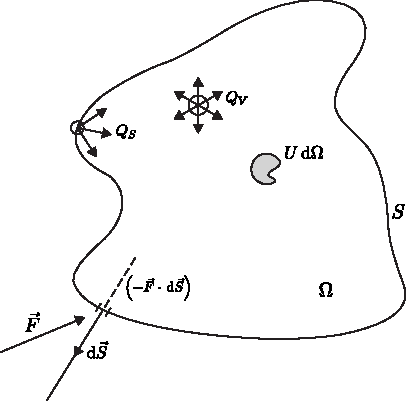
\includegraphics{conservationscheme}
	% If not, use
	%\picplace{5cm}{2cm} % Give the correct figure height and width in cm
	%
	\caption{Ley de conservación para una magnitud escalar.
		Adaptado de~\cite{Hirsch2007}.}
	\label{fig:1}       % Give a unique label
\end{figure}
Simplificamos~\eqref{eq:integralbalance} utilizando el teorema de la
divergencia de Gauß en la integral de superficie para obtener
\begin{equation}\label{eq:integralbalance2}
	\diff{}{t}
	\int_{\omega}
	\mathbf{U}\dl{\mathbf{x}}
	+\int_{\omega}
	\operatorname{div}
	\left(\mathbf{F}\right)
	\dl{\mathbf{x}}=
	\int_{\omega}
	\mathbf{S}\dl{\mathbf{x}}.
\end{equation}
Dado que~\eqref{eq:integralbalance2} se cumple para cualquier
subdominio $\omega\subset\Omega$,
\begin{equation}\label{eq:balancelaw}
	\forall\left(x,t\right)\in\Omega\times\mathbb{R}_{+}:
	\diffp{\mathbf{U}}{t}+
	\operatorname{\operatorname{div}
		\left(\mathbf{F}\right)}=
	\mathbf{S}.
\end{equation}
La ecuación~\eqref{eq:balancelaw} se llama \emph{ley de balance}.
Frequentemente, el único cambio en $\mathbf{U}$ proviene de los
flujos y la fuente se fija en cero.
\begin{equation}\label{eq:conservationlaw}
	\forall\left(x,t\right)\in
	\Omega\times\mathbb{R}_{+}:
	\diffp{\mathbf{U}}{t}+
	\operatorname{\operatorname{div}
		\left(\mathbf{F}\right)}=
	0.
\end{equation}
La ecuación~\eqref{eq:conservationlaw} se llama
\emph{ley de conservación}, ya que el único cambio en $\mathbf{U}$
procede de la cantidad que entra o sale del dominio de interés.

\section*{Ejemplos de leyes de conservación}

Algunos ejemplos de leyes de conservación son la ecuación de
transporte escalar, la ecuación de difusión, las ecuaciones de Euler,
la ecuación de Richards y la ecuación Buckley-Leverett.

\subsection*{Ecuación de transporte escalar}

Sea $\mathbf{U}=U$ la concentración de un contaminante en un río.
Suponga que el río fluye con un campo de velocidad
$\mathbf{a}\left(\mathbf{x},t\right)$ y conocemos el campo de
velocidad en todos los puntos del río.
El contaminante es transportado en la dirección de la velocidad, y
así el flujo es $\mathbf{F}=\mathbf{a}U$.
Dado que no hay producción ni destrucción del contaminante durante el
flujo, el término fuente en~\eqref{eq:balancelaw} es cero.
La ley de conservación~\eqref{eq:conservationlaw} resulta ser
\begin{equation}
	\diffp{U}{t}+
	\operatorname{div}
	\left(\mathbf{a}\left(\mathbf{x},t\right)U\right)=
	0.
\end{equation}

\subsection*{Ecuación de difusión}

Sea $\mathbf{U}=U$ la temperatura de un bloque metálico.
Suponga que el bloque se calienta por un extremo y se deja enfriar
después, sin aportar ninguna fuente de calor adicional.
El calor se propaga o difunde y la temperatura del bloque se
uniformiza al cabo de un tiempo.
La difusión del calor se rige por la ley de Fick
\begin{equation}\label{eq:ficklaw}
	\mathbf{F}\left(U\right)=
	-\mathbf{k}\nabla U.
\end{equation}
Aquí, $\mathbf{k}$ es el tensor de conductividad del medio.
Sustituyendo~\eqref{eq:ficklaw} en~\eqref{eq:conservationlaw}
resulta ser
\begin{equation}
	\diffp{U}{t}-
	\operatorname{div}
	\left(\mathbf{k}\nabla U\right)=
	0.
\end{equation}

\subsection*{Ecuaciones de Euler}

El aire consiste de un gran número de moléculas.
El movimiento de cada molécula puede seguirse individualmente y
da lugar a un gran número de EDOs.
El sistema EDO resultante es demasiado grande para ser
computacionalmente viable.
En su lugar, se utiliza una descripción macroscópica de un gas ideal
y se ignora los efectos de viscosidad y la conducción de calor.
Las variables de interés son la densidad $\rho$, el campo de
velocidad $\mathbf{u}$ y la presión del gas $p$.
Las leyes de conservación relevante son

\begin{description}
	\item[\bfseries Conservación de la masa]

	      La masa total de un gas es conservado, garantizado
	      por el Teorema de la circulación de
	      Kelvin~\cite[pág. 28]{Wesseling2001}.
	      % https://en.wikipedia.org/wiki/Kelvin%27s_circulation_theorem

	\item[\bfseries Conservación de la cantidad de movimiento]

	      Se sigue de la segunda ley de Newton que la tasa de cambio de
	      la cantidad de movimiento es igual a la fuerza aplicada.
	      En ausencia de fuerzas externas, la presión del gas es la
	      única fuerza que actúa sobre el gas.

	\item[\bfseries Conservación de la energía]

	      La suma de la energía cinética y de la energía interna
	      (potencial) del gas ideal es la energía total
	      \begin{math}
		      E=
		      \frac{p}{\gamma-1}+
		      \frac{1}{2}
		      \rho{\left|\mathbf{u}\right|}^{2}
	      \end{math},
	      donde la constante del gas $\gamma$ es $\frac{5}{3}$ si este
	      es monoatómico y $\frac{7}{5}$ si es diatómico.
\end{description}

Estas tres leyes de conservación forman un sistema EDP no lineal
llamado las ecuaciones de Euler para la dinámica de gases.
\begin{align}
	\diffp{\rho}{t}+
	\operatorname{div}
	\left(\rho\mathbf{u}\right)             & =
	0.                                          \\
	\diffp{\rho\mathbf{u}}{t}+
	\operatorname{div}
	\left(\rho\mathbf{u}\otimes\mathbf{u}\right)+
	\nabla p                                & =
	0.                                          \\
	\diffp{E}{t}+
	\operatorname{div}
	\left(\left(E+p\right)\mathbf{u}\right) & =
	0.
\end{align}

Para cualquier
\begin{math}
	a=
	\begin{bmatrix}
		a_{1} \\
		a_{2} \\
		a_{3}
	\end{bmatrix},
	b=
	\begin{bmatrix}
		b_{1} \\
		b_{2} \\
		b_{3}
	\end{bmatrix}\in\mathbb{R}^{3}
\end{math}
se define el producto tensorial como
\begin{equation*}
	a\otimes b\coloneqq
	\begin{bmatrix}
		a_{1}b_{1} & a_{1}b_{2} & a_{1}b_{3} \\
		a_{2}b_{1} & a_{2}b_{2} & a_{2}b_{3} \\
		a_{3}b_{1} & a_{3}b_{2} & a_{3}b_{3} \\
	\end{bmatrix}\in\mathbb{R}^{3\times 3}.
\end{equation*}

\subsection*{Ecuación de Richards}

Derivada la conservación de la masa, la ecuación de continuidad
unidimensional de la infiltración se da como~\cite{Tan2018}
\begin{equation}\label{eq:reynoldstheorem}
	\diffp{\theta}{t}+
	\operatorname{div}\left(\mathbf{q}\right)=
	0.
\end{equation}
Por la ley de Darcy, $q_{z}$ representa
\begin{equation}\label{eq:darcy}
	q_{z}=
	-K\diffp{H}{z}=
	-K\diffp{\left(h-z\right)}{z}=
	K\left(
	1-
	\diffp{h}{z}
	\right).
\end{equation}
Uniendo las ecuaciones~\eqref{eq:reynoldstheorem} y~\eqref{eq:darcy}
obtenemos la formulación mixta de Richards
\begin{equation*}
	\frac{\partial\theta}{\partial t}+
	\frac{\partial}{\partial z}
	\left[K\left(1-\frac{\partial h}{\partial z}\right)\right]=0.
\end{equation*}
donde
\begin{itemize}
	\item

	      $\theta$ es el contenido de agua del suelo $\left(\unit[per-mode=symbol]{\cubic\metre\per\cubic\metre}\right)$.

	\item

	      $z$ es la profundidad del suelo.

	\item

	      $\mathbf{q}$ es la tasa de infiltración de agua $\left(\unit[per-mode=symbol]{\metre\per\second}\right)$.

	\item

	      $K$ es la conductividad hidráulica.

	\item

	      $H$ es el potencial hídrico total en el eje $z$.

	\item

	      $h$ es la cabeza de presión\footnote{\url{https://en.wikipedia.org/wiki/Pressure_head}}.
\end{itemize}

\subsection*{Ecuación de Buckley-Leverett}

La ecuación de Buckley-Leverett definida por la ley de conservación
con
\begin{equation*}
	f\left(u\right)=
	\frac{\mu u^{2}}{\mu u^{2}+{\left(1-\mu\right)}^{2}}
\end{equation*}
provee un modelo simple para el flujo de dos fluidos inmiscibles en
un medio poroso y tiene aplicaciones en la simulación de yacimientos
petrolíferos.
La solución representa la saturación de agua en un yacimiento de
petróleo y $0<\mu<1$ representa la movilidad.

\subsection*{Ecuaciones de Saint-Venant}

Consideremos el flujo de agua con una superficie libre bajo gravedad
en un dominio tridimensional, donde $xy$ determinan un plano
horizontal y $z$ definen la dirección vertical, que asociamos con la
elevación de la superficie libre.
La región de interés se encuentra por encima de un punto de
referencia horizontal en $z=0$.
El fluido se encuentra por encima de la elevación del fondo del canal
$b\left(x\right)\geq 0$; la pendiente $\diff{b\left(x\right)}{x}$ de
la elevación del fondo da lugar a un término fuente en las
ecuaciones; $h\left(x,t\right)$ es la profundidad del flujo;
$u\left(x,t\right)$ es la velocidad de la partícula; la superficie
libre está bajo la influencia de la aceleración de la gravedad $g$.
Suponemos una batimetría variable $z=b\left(x,y\right)$ y la
superficie libre es
\begin{math}
	z=
	s\left(x,y,t\right)=
	b\left(x,y\right)+
	h\left(x,y,t\right)
\end{math}.
Asumiendo que la densidad del fluido es constante~\cite{Toro2024}.

\begin{align*}
	\diffp{h}{t}+
	u\diffp{h}{x}+
	h\diffp{u}{x}+
	v\diffp{h}{y}+
	h\diffp{v}{y} & =0. \\
	\diffp{u}{t}+
	u\diffp{u}{x}+
	g\diffp{h}{x}+
	v\diffp{u}{y}+
	g\diffp{b}{x} & =
	0.                  \\
	\diffp{v}{t}+
	u\diffp{v}{x}+
	v\diffp{v}{y}+
	g\diffp{h}{y}+
	g\diffp{b}{y} & =
	0.
\end{align*}
Donde $h\left(x,y,t\right)$, $u\left(x,y,t\right)$ y
$v\left(x,y,t\right)$ son la profundidad, la componente de velocidad
$x$ y la componente de velocidad $y$, respectivamente.
La elevación del lecho sobre un dato horizontal viene dada por la
función $b\left(x,y\right)$, que se supone prescrita; $g$ denota la
aceleración de la gravedad.

\begin{figure}[b]
	\sidecaption[t]
	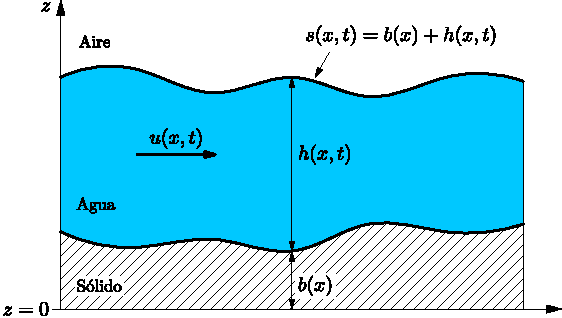
\includegraphics{saintvenant}
	\caption{Vista lateral del montaje físico para las ecuaciones de Saint-Venant.
		La capa de agua se encuentra entre el fondo impermeable ($b(x)$ sobre
		un punto de referencia horizontal ($z=0$)) y la superficie libre
		($s(x,t)=b(x)+h(x,t)$).}
	\label{fig:2}
\end{figure}

\subsection*{Ecuación de Burgers no viscosa}

El ejemplo más conocido de una ley de conservación no lineal es la
ecuación de Burgers~\cite{Burgers1995} no viscosa definida con
\begin{equation*}
	f\left(u\right)=
	\frac{1}{2}u^{2}.
\end{equation*}
Este es un modelo simplificado para entender el comportamiento no
lineal del flujo de tráfico de autos en una autopista y la formación
de atascos.
Para profundizar en los modelos presentados vea~\cite{Vázquez2015}.

% \section{Antecedentes}
% \label{sec:1}
% Use the template \emph{chapter.tex} together with the

% \section{Trabajos relacionados}
% \section{Modelo de leyes de conservación}
% \label{sec:2}

% Always give a unique label
% and use \ref{<label>} for cross-references
% and \cite{<label>} for bibliographic references
% use \sectionmark{}
% to alter or adjust the section heading in the running head

% \eject

% \begin{eqnarray}
% 	\left|\nabla U_{\alpha}^{\mu}(y)\right| &\le&\frac1{d-\alpha}\int
% 	\left|\nabla\frac1{|\xi-y|^{d-\alpha}}\right|\,d\mu(\xi) =
% 	\int \frac1{|\xi-y|^{d-\alpha+1}} \,d\mu(\xi)\qquad  \\
% 	&=&(d-\alpha+1) \int\limits_{d(y)}^\infty
% 	\label{eq:01}
% \end{eqnarray}

% \enlargethispage{24pt}

% \subsection{Modelo de Burgers}
% \label{subsec:2}
% Instead of simply listing\index{cross-references} and citations\index{citations} as has already been described in Sect.~\ref{sec:2}.

% \begin{quotation}
% 	Please do not use quotation marks when quoting texts! Simply use the \verb|quotation| environment -- it will automatically be rendered in the preferred layout.
% \end{quotation}

% \subsection{Buckley-Leverett}

% \paragraph{Paragraph Heading} %
% Instead of simply listing headings of different levels we recommend to let every heading be followed by at least a short passage of text. Furtheron please use the \LaTeX\ automatism for all your cross-references and citations as has already been described in Sect.~\ref{sec:2}.

% \begin{enumerate}
% 	\item{Livelihood and survival mobility are oftentimes coutcomes of uneven socioeconomic development.}
% \end{enumerate}


% \subparagraph{Subparagraph Heading} In order to avoid simply listing headings of different levels we recommend to let every heading be followed by at least a short passage of text. Use the \LaTeX\ automatism for all your cross-references and citations as has already been described in Sect.~\ref{sec:2}, see also Fig.~\ref{fig:2}.

% Please note that the first line of text that follows a heading is not indented, whereas the first lines of all subsequent paragraphs are.

% \begin{itemize}
% 	\item{Livelihood and survival mobility are oftentimes coutcomes of uneven socioeconomic development, cf. Table~\ref{tab:1}.}
% \end{itemize}

% \runinhead{Run-in Heading Boldface Version} Use the \LaTeX\ automatism for all your cross-references and citations as has already been described in Sect.~\ref{sec:2}.

% \subruninhead{Run-in Heading Boldface and Italic Version} Use the \LaTeX\ automatism for all your cross-refer\-ences and citations as has already been described in Sect.~\ref{sec:2}\index{paragraph}.

% \subsubruninhead{Run-in Heading Displayed Version} Use the \LaTeX\ automatism for all your cross-refer\-ences and citations as has already been described in Sect.~\ref{sec:2}\index{paragraph}.
% % Use the \index{} command to code your index words
% %
% % For tables use
% %
% \begin{table}[!t]
% 	\caption{Please write your table caption here}
% 	\label{tab:1}       % Give a unique label
% 	%
% 	% For LaTeX tables use
% 	%
% 	\begin{tabular}{p{2cm}p{2.4cm}p{2cm}p{4.9cm}}
% 		\hline\noalign{\smallskip}
% 		Classes     & Subclass & Length      & Action Mechanism                      \\
% 		\noalign{\smallskip}\svhline\noalign{\smallskip}
% 		Translation & mRNA$^a$ & 22 (19--25) & Translation repression, mRNA cleavage \\
% 		\noalign{\smallskip}\hline\noalign{\smallskip}
% 	\end{tabular}
% 	$^a$ Table foot note (with superscript)
% \end{table}
%
% \section{Contenido principal y organización}
% \label{sec:3}
% % Always give a unique label
% % and use \ref{<label>} for cross-references
% % and \cite{<label>} for bibliographic references
% % use \sectionmark{}
% % to alter or adjust the section heading in the running head
% Instead of simply listing headings of different levels we recommend to let every heading be followed by at least a short passage of text. Furtheron please use the \LaTeX\ automatism for all your cross-references and citations as has already been described in Sect.~\ref{sec:2}.

% If you want to list definitions or the like we recommend to use the Springer-enhanced \verb|description| environment -- it will automatically render Springer's preferred layout.

% \begin{description}[Type 1]
% 	\item[Type 1]{That addresses central themes pertainng to migration, health, and disease. In Sect.~\ref{sec:1}, Wilson discusses the role of human migration in infectious disease distributions and patterns.}
% 	\item[Type 2]{That addresses central themes pertainng to migration, health, and disease. In Sect.~\ref{subsec:2}, Wilson discusses the role of human migration in infectious disease distributions and patterns.}
% \end{description}

% \begin{svgraybox}
% 	If you want to emphasize complete paragraphs of texts we recommend to use the newly defined Springer class option \verb|graybox| and the newly defined environment \verb|svgraybox|. This will produce a 15 percent screened box 'behind' your text.

% 	If you want to emphasize complete paragraphs of texts we recommend to use the newly defined Springer class option and environment \verb|svgraybox|. This will produce a 15 percent screened box 'behind' your text.
% \end{svgraybox}

% \begin{theorem}
% 	Theorem text goes here.
% \end{theorem}

% \begin{definition}
% 	Definition text goes here.
% \end{definition}

% \begin{proof}
% 	%\smartqed
% 	Proof text goes here.
% 	%\qed
% \end{proof}

% \paragraph{Paragraph Heading} %
% Instead of simply listing headings of different levels we recommend to let every heading be followed by at least a short passage of text. Furtheron please use the \LaTeX\ automatism for all your cross-references and citations as has already been described in Sect.~\ref{sec:2}.

% \begin{trailer}{Trailer Head}
% 	If you want to emphasize complete paragraphs of texts in a \verb|Trailer Head| we recommend to
% 	use  \begin{verbatim}\begin{trailer}{Trailer Head}
% ...
% \end{trailer}\end{verbatim}
% \end{trailer}
% %
% \begin{questype}{Questions}
% 	If you want to emphasize complete paragraphs of texts in an \verb|Questions| we recommend to
% 	use  \begin{verbatim}\begin{questype}{Questions}
% ...
% \end{questype}\end{verbatim}
% \end{questype}
% %
% %
% \begin{important}{Important}
% 	If you want to emphasize complete paragraphs of texts in an \verb|Important| we recommend to
% 	use  \begin{verbatim}\begin{important}{Important}
% ...
% \end{important}\end{verbatim}
% \end{important}
% %
% \clearpage
% \begin{warning}{Attention}
% 	If you want to emphasize complete paragraphs of texts in an \verb|Attention| we recommend to
% 	use  \begin{verbatim}\begin{warning}{Attention}
% ...
% \end{warning}\end{verbatim}
% \end{warning}

% \begin{programcode}{Program Code}
% 	If you want to emphasize complete paragraphs of texts in a \verb|Program Code| we recommend to
% 	use

% 	\verb|\begin{programcode}{Program Code}|

% 	\verb|\begin{verbatim}...\end{verbatim}|

% 	\verb|\end{programcode}|

% \end{programcode}
% %
% \begin{tips}{Tips}
% 	If you want to emphasize complete paragraphs of texts in a \verb|Tips| we recommend to
% 	use  \begin{verbatim}\begin{tips}{Tips}
% ...
% \end{tips}\end{verbatim}
% \end{tips}
% %
% %
% \begin{overview}{Overview}
% 	If you want to emphasize complete paragraphs of texts in an \verb|Overview| we recommend to
% 	use  \begin{verbatim}\begin{overview}{Overview}
% ...
% \end{overview}\end{verbatim}
% \end{overview}
% \clearpage
% \begin{backgroundinformation}{Background Information}
% 	If you want to emphasize complete paragraphs of texts in a \verb|Background|
% 	\verb|Information| we recommend to
% 	use

% 	\verb|\begin{backgroundinformation}{Background Information}|

% 	\verb|...|

% 	\verb|\end{backgroundinformation}|
% \end{backgroundinformation}
% \begin{legaltext}{Legal Text}
% 	If you want to emphasize complete paragraphs of texts in a \verb|Legal Text| we recommend to
% 	use  \begin{verbatim}\begin{legaltext}{Legal Text}
% ...
% \end{legaltext}\end{verbatim}
% \end{legaltext}
% %
% \begin{acknowledgement}
% 	If you want to include acknowledgments of assistance and the like at the end of an individual chapter please use the \verb|acknowledgement| environment -- it will automatically render Springer's preferred layout.
% \end{acknowledgement}

\chapter{Leyes de conservación hiperbólicas escalares}

Se define la ley de conservación escalar como
\begin{equation}\label{eq:1}
	\diffp{u}{t}+
	\diffp{f\left(u\right)}{x}=
	0.
\end{equation}
donde $u\left(x,t\right)$ es la función desconocida y $f$ es la
función flujo.
Reescriba~\eqref{eq:1} en la forma integral
\begin{equation}\label{eq:2}
	\forall a,b\in\mathbf{R}:
	\diff{}{t}
	\int_{a}^{b}
	u\left(x,t\right)
	\dl x+
	f\left(u\left(b,t\right)\right)-
	f\left(u\left(a,t\right)\right)=0.
\end{equation}
Decimos que $u$ es una solución débil si y solamente si satisface~\eqref{eq:2}
para casi todos los $a,b\in\mathbb{R}$.
Equivalentemente, $u$ es una solución débil si y solamente si
\begin{equation*}
	\forall\varphi\in C^{1}_{0}\left(\mathbf{R}\times\left[0,\infty\right)\right)
	-\int_{0}^{\infty}
	\int_{-\infty}^{\infty}
	\left[u\diffp{\varphi}{t}+
		f\left(u\right)\diffp{\varphi}{x}\right]
	\dl x\dl t-
	\int_{-\infty}^{\infty}
	u^{0}\left(x\right)\varphi\left(x,0\right)
	\dl x=0.
\end{equation*}

\section{Condición de Rankine-Hugoniot}

En~\eqref{eq:2}, considere dos segmentos de clase $C^{1}$ separados
por una curva $x=x\left(t\right)$.
\begin{equation*}
	\diff{}{t}
	\left(
	\underbrace{
		\int_{a}^{x\left(t\right)}
		u\left(x,t\right)
		\dl x
	}_{\coloneqq G_{a}\left(x\left(t\right),t\right)}+
	\underbrace{
		\int_{x\left(t\right)}^{b}
		u\left(x,t\right)
		\dl x
	}_{\coloneqq G_{b}\left(x\left(t\right),t\right)}
	\right)+
	f\left(u\left(b, t\right)\right)-
	f\left(u\left(a,t\right)\right)=
	0.
\end{equation*}

\begin{align*}
	\diff{G_{a}}{t} & =
	\diffp{G_{a}}{x}\cdot
	\diff{x}{t}+
	\diffp{G_{a}}{t}.   \\
	\diff{G_{a}}{t} & =
	u\left(x\left(t\right),t\right)
	\diff{x}{t}+
	\int_{a}^{x\left(t\right)}
	\diffp{u}{t}
	\dl x.              \\
	\diff{G_{a}}{t} & =
	u\left(x\left(t\right),t\right)\diff{x}{t}-
	\int_{a}^{x\left(t\right)}
	\diffp{f\left(u\right)}{x}
	\dl x.
\end{align*}
y análogamente para $\diff{G_{b}}{t}$.
Debido a la discontinuidad en $u\left(x\left(t\right),t\right)$,
$\diff{G_{a}}{t}$ no existe.
Pero, los límites laterales son
\begin{align*}
	\left[
		\frac{dG_a(x(t), t)}{t}
	\right]^- & =
	u^-
	x'(t)-
	(f(u^-)-
	f(u(a, t))).  \\
	\left[
		\frac{dG_b(x(t), t)}{t}
	\right]^+ & =
	-u^+
	x'(t)-
	(f(u(b, t))-
	f(u^+)).
\end{align*}
Defina $u^{-}\coloneqq u\left(x\left(t\right)^-, t\right)$,
$u^{+}\coloneqq u\left(x\left(t\right)^{+},t\right)$.
Reemplace en la forma integral $u^-x'\left(t\right)-f(u^-)-u^+x'(t)+f\left(u^{+}\right)=0$
y obtenga la condición de Rankine-Hugoniot.
\begin{equation}
	\diff{x\left(t\right)}{t}=
	\frac{f\left(u^{+}\right)-f\left(u^{-}\right)}{u^{+}-u^{-}}
\end{equation}

\begin{theorem}
	Si $u$ es seccionalmente de clase $C^{1}$ y discontinua solo a lo largo
	de curvas aisladas, $u$ satisface la EDP y la condición de Rankine-Hugoniot
	a lo largo de todas las curvas discontinuas, entonces $u$ es una solución débil
	de la ley de conservación.
\end{theorem}

\begin{example}
	Considere el problema de Riemann
	\begin{equation*}
		\begin{cases}
			\diffp{u}{t}+
			\diffp{}{x}
			\left(\frac{u^{2}}{2}\right)=
			0. \\
			u\left(x,0\right)=
			\begin{cases}
				1  & x < 0.    \\
				-1 & x \geq 0.
			\end{cases}
		\end{cases}
	\end{equation*}
\end{example}
La condición inicial simplemente se propaga en el tiempo
(a ``velocidad $0$'') para formar una solución débil (un choque).

\begin{example}
	Considere el problema de Riemann
	\begin{equation*}
		\begin{cases}
			\diffp{u}{t}+
			\diffp{}{x}
			\left(\frac{u^{2}}{2}\right)=
			0. \\
			u\left(x,0\right)=
			\begin{cases}
				-1 & x < 0.    \\
				1  & x \geq 0.
			\end{cases}
		\end{cases}
	\end{equation*}
	la condición inicial propagada también forma una solución débil.
	Pero, considere
	\begin{equation*}
		u\left(x,t\right)=
		\begin{cases}
			-1          & x \leq -t.  \\
			\frac{x}{t} & -t < x < t. \\
			1           & x > t.
		\end{cases}
	\end{equation*}
	También es una solución débil (onda de rarefacción).
\end{example}

Decimos que una onda de propagación discontinua con rapidez $s$
satisface la condición de entropía si y solamente si
\begin{equation*}
	f^{\prime}\left(u^{-}\right)>s>f^{\prime}\left(u^{+}\right).
\end{equation*}
Si $f$ es convexa, entonces $f^{\prime}$ es monótona decreciente y la rapidez
$s$ verifica la condición de entropía.
Las características de estas ondas de propagación son
\begin{itemize}
	\item

	      constante a lo largo de las trayectorias de las partículas,

	\item

	      en flujo suave esta onda salta a valores más altos durante un
	      choque.
\end{itemize}

\begin{definition}
	Una entropía $\eta\left(u\right)$ y un flujo de entropía
	$\psi\left(u\right)$ son funciones tal que $\eta$ es convexa y
	\begin{math}
		\diffp{\eta\left(u\right)}{t}+
		\diffp{\psi\left(u\right)}{x}=
		0
	\end{math}
	para soluciones suaves de una ley de conservación.
\end{definition}

Para encontrar $\eta\left(u\right)$ y $\psi\left(u\right)$ que satisfaga
\begin{math}
	\diffp{\eta\left(u\right)}{t}+
	\diffp{\psi\left(u\right)}{x}=0
\end{math}.
Para $u$ suave, la regla de la cadena da
\begin{math}
	\eta^{\prime}
	\left(u\right)
	\diffp{u}{t}+
	\psi^{\prime}\left(u\right)
	\diffp{u}{x}=
	0
\end{math}.
Similarmente, reescriba la ley de conservación
\begin{align*}
	\diffp{u}{t}+
	f^{\prime}\left(u\right)
	\diffp{u}{x} & =0. \\
	\eta^{\prime}\left(u\right)
	\diffp{u}{t}+
	\eta^{\prime}\left(u\right)
	f^{\prime}\left(u\right)
	\diffp{u}{x} & =
	0.
\end{align*}
Esto nos da
\begin{math}
	\psi^{\prime}
	\left(u\right)=
	-\eta^{\prime}
	\left(u\right)
	\frac{\diffp{u}{t}}{\diffp{u}{x}}=
	\eta^{\prime}\left(u\right)
	f^{\prime}\left(u\right)
\end{math}.

\begin{example}[Par entropía-flujo de la ecuación de Burgers]
	Sea el flujo $f\left(u\right)=\frac{u^{2}}{2}$.
	Si $\eta\left(u\right)=u^{2}$, entonces
	$\psi^{\prime}\left(u\right)=2u\cdot u$, es decir,
	$\psi\left(u\right)=\frac{2}{3}u^{3}$.
\end{example}

\begin{definition}
	La función $u\left(x,t\right)$ es una solución de entropía
	de la ley de conservación si y solamente si
	para toda las funciones de entropía convexas y su correspondiente flujo de entropía
	satisface la desigualdad
	\begin{equation*}
		\diffp{\eta\left(u\right)}{t}+
		\diffp{\psi\left(u\right)}{x}=
		0.
	\end{equation*}
\end{definition}

Nuevamente, considere la ecuación de Burgers e integre sobre el rectángulo
$\left[x_{1},x_{1}+\Delta x\right]\times\left[t_{1},t_{1}+\Delta t\right]$.

\begin{align*}
	0 & \geq
	\left[
		\int_{x_{1}}^{x_{1}+\Delta x}
		u^{2}\right]_{t_1}^{t_1+\Delta t}+
	\left[
	\int_{t_{1}}^{t_{1}+\Delta t}
	\frac{2}{3}u^{3}
	\right]_{x_{1}}^{x_{1}+\Delta x}     \\
	  & =
	s_{1}\Delta t
	\left(u_{1}^{2}-u_{r}^{2}\right)+
	\frac{2}{3}
	\Delta t
	\left(u_{r}^{3}-u_{1}^{3}\right)+
	\mathcal{O}(\Delta t^{2}).           \\
	  & =
	\Delta t
	\left(u_{1}^{2}-u_{r}^{2}\right)
	\left(s_{1}-s_{2}\right)+
	\mathcal{O}\left(\Delta t^{2}\right) \\
	  & =
	-\frac{1}{6}
	\left(u_{l}-u_{r}\right)^{3}
	\Delta t+
	\mathcal{O}\left(\Delta t^{2}\right)
	\quad\to\quad
	u_{l}>u_{r}.                         \\
\end{align*}
con $s_{1}=\frac{\left[\frac{u^{2}}{2}\right]}{\left[u\right]}$,
$s_{2}=\frac{\left[\frac{2}{3}u^{3}\right]}{\left[u^{2}\right]}$,
$s_{2}-s_{1}=\frac{\left[u\right]^{2}}{6\left(u_{l}+u_{r}\right)}$.

\begin{definition}
	La variación total de $u$ se define como
	\begin{equation*}
		\operatorname{TV}\left(u\right)\coloneqq
		\limsup_{\varepsilon\to0}
		\frac{1}{\varepsilon}
		\int
		\left|
		u\left(x+\varepsilon\right)-
		u\left(x\right)
		\right|\dl x.
	\end{equation*}
	Además, si $u$ es diferenciable, entonces
	\begin{equation*}
		\operatorname{TV}\left(u\right)\coloneqq
		\int\left|u^{\prime}\left(x\right)\right|\dl x.
	\end{equation*}
\end{definition}

\begin{theorem}
	Sea $u$ una solución de una ley de conservación con
	$f^{\prime\prime}\left(u\right)\geq 0$.
	Entonces,
	\begin{equation*}
		\forall\Delta t\geq 0:
		\operatorname{TV}
		\left(u\left(t+\Delta t,\cdot\right)\right)\leq
		\operatorname{TV}
		\left(u\left(t,\cdot\right)\right).
	\end{equation*}
\end{theorem}

% \section*{Modelo de flujo de tráfico}

% \begin{equation}
% 	\diffp{U}{t}+
% 	\diffp{V_{\text{max}}U\left(1-U\right)}{x}=
% 	0.
% \end{equation}

% \section*{Recuperación mejorada de petróleo}

% \begin{equation}
% 	\diffp{S^{\text{oil}}}{t}+
% 	\diffp{
% 		\frac{q\left(S^{\text{oil}}\right)^{2}}{\left(S^{\text{oil}}\right)^{2}+\left(1-S^{\text{oil}}\right)^{2}}
% 	}{x}=
% 	0.
% \end{equation}

% \section*{Condición de salto de Rankine-Hugoniot}

% \section*{Solución al problema de Riemann}

% Una función
% $U\in L^{\infty}\left(\mathbb{R}\times\mathbb{R}_{+}\right)$
% es una solución entrópica


% \section{Problema de Riemann}
% \section{Solución débil}
% \section{Función entrópica}
% \section{Condición de Rankine-Hugoniot}
% \section{Teorema de Lax-Wendroff}

\chapter{Método de Volúmenes Finitos}

\abstract{
	El método de los volúmenes finitos constituye una técnica
	numérica robusta para aproximar la solución de un problema de
	valor inicial frontera de una ley de conservación
	\begin{math}
		\difcp{u}{t}+
		\difcp{f\left(u\right)}{x}=
		0
	\end{math},
	por funciones constantes por partes~\cite[p.~5]{Saeed2025}.
	Este enfoque se basa en discretizar el dominio computacional
	$\Omega\subset\mathbb{R}^{d}$ en una malla compuesta por celdas
	disjuntas
	\begin{math}
		\Omega^{h}=
		\bigcup_{j=1}^{N}
		\Omega_{j}
	\end{math},
	cuya unión cubre el dominio salvo un conjunto de medida nula.
	Para transformar el problema continuo en un sistema algebraico
	discreto, integre la EDP sobre cada celda $\Omega_{j}$.
	Las incógnitas del sistema son aproximaciones del valor medio de
	la solución en cada celda, lo que preserva localmente las
	propiedades de conservación de la EDP.
}

\begin{figure}[ht!]
	\centering
	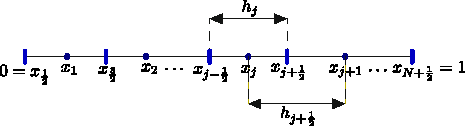
\includegraphics[width=.45\textwidth]{fv1d}
	\caption{
	Malla de volúmenes finitos 1D de $\Omega=\left(0,1\right)$.
	Los nodos de índices fraccionarios
	\begin{math}
		{\big\{x_{j\pm\frac{1}{2}}\big\}}^{N}_{j=1}
	\end{math}
	son los extremos de las celdas
	\begin{math}
		\Omega_{j}=
		\big[
			x_{j-\frac{1}{2}},
			x_{j+\frac{1}{2}}
			\big]
	\end{math}
	cuyo tamaño es $h_{j}$, y los nodos de índices enteros
	\begin{math}
		{\big\{x_{j}\big\}}^{N}_{j=1}
	\end{math}
	son los centros de las celdas.
	Si $x_{0}=-x_{1}$ y $x_{N+1}=2-x_{N}$, entonces $h_{0}=h_{1}$ y
	$h_{N+1}=h_{N}$.
	La distancia entre dos celdas consecutivas es
	\begin{math}
		h_{j+\frac{1}{2}}=
		\frac{1}{2}\left(h_{j}+h_{j+1}\right),
		\forall j=0,\dotsc,N
	\end{math}.
	}
\end{figure}

\section{La ecuación de Poisson unidimensional}

Nuestra presentación de los métodos de volúmenes finitos fue
fuertemente influenciado
por~\cite{Adler2025,Eymard2000,Hesthaven2018,LeDret2016}.
También remitimos al lector a textos más centrados en la ecuación
de Poisson, tales como~\cite[p.~337]{Choksi2022},
\cite[p.~22]{Evans2010} y~\cite[p.~29]{Hackbusch2017}.
\begin{align}
	\shortintertext{
		Sea
		\begin{math}
			\Omega=
			\left(0,1\right)\subset
			\mathbb{R}
		\end{math}.
		Encuentre una solución
		\begin{math}
			u\in
			C^{2}\left(\Omega\right)\cap
			C^{0}\big(\overline{\Omega}\big)
		\end{math}
		que satisfaga el siguiente problema elíptico con condiciones de
		frontera Dirichlet homogénea~\eqref{eq:PoissonBVP}, donde
		\begin{math}
			f\in
			C^{0}\big(\overline{\Omega}\big)
		\end{math}.
	}
	\begin{cases}
		-\difc.L.{}{}u=f &
		\text{en }\Omega.  \\
		u=0              &
		\text{en }\partial\Omega.
	\end{cases}\label{eq:PoissonBVP}
	\shortintertext{
		Suponga que $\Omega^{h}=\bigcup^{N}_{j=1}\Omega_{j}$ es una
		malla de volúmenes finitos de $\Omega$.
		Integra la EDP~\eqref{eq:PoissonBVP} en $\Omega_{j}$ y emplea
		el teorema fundamental del cálculo, obtenga
	}
	\forall j=1,\dotsc,N:
	-\diff{u}{x}[x_{j+\frac{1}{2}}]+
	\diff{u}{x}[x_{j-\frac{1}{2}}] & =
	-\int_{\Omega_{j}}
	\diff[2]{u\left(x\right)}{x}
	\dl x=
	\int_{\Omega_{j}}
	f\left(x\right)\dl x.\label{eq:PoissonBVPIntegral}
	\shortintertext{
		Sea
		\begin{math}
			h=
			\max
			\left\{
			h_{j}\mid 0\leq j\leq N
			\right\}
		\end{math}
		y dado que
		\begin{math}
			u\in
			C^{2}\left(\Omega\right)
		\end{math},
		por el teorema de Taylor en la celda $\Omega_{j}$ se tiene
	}\label{eq:Taylor}
	\forall j=1,\dotsc,N:
	u\big(x_{j+\frac{1}{2}}\big)+
	\big(x-x_{j+\frac{1}{2}}\big)
	\diff{u}{x}[x_{j+\frac{1}{2}}]+
	\mathcal{O}\big(h^{2}\big)     & =
	u\left(x\right).
	\shortintertext{
	Use la condición de frontera $u\big(x_{\frac{1}{2}}\big)=0$
	en~\eqref{eq:Taylor} e integre sobre $\Omega_{1}$.
	}
	{\bigg[
	\frac{x^{2}}{2}-x_{\frac{1}{2}}x
	\bigg]}^{x_{\frac{3}{2}}}_{x_{\frac{1}{2}}}
	\diff{u}{x}[x_{\frac{1}{2}}]
	\dl x+
	\mathcal{O}\big(h^{3}\big)     & =
	\int_{\Omega_{1}}
	u\left(x\right)
	\dl x.\notag                             \\
	\diff{u}{x}[x_{\frac{1}{2}}]   & \approx
	\frac{1}{h_{\frac{1}{2}}}
	\left[
		\frac{1}{h_{1}}
		\int_{\Omega_{1}}
		u\left(x\right)
		\dl x
		\right].\notag
	% 	\forall j=1,\dotsc,N-1:
	% \diff{u}{x}[x_{j+\frac{1}{2}}] & \approx
	% 	\frac{1}{h_{j+\frac{1}{2}}}
	% 	\left[
	% 		\frac{1}{h_{j+1}}
	% 		\int_{\mathclap{\Omega_{j+1}}}
	% 		u\left(x\right)
	% 		\dl x-
	% 		\frac{1}{h_{j}}
	% 		\int_{\Omega_{j}}
	% 		u\left(x\right)
	% 		\dl x
	% \right].\notag                           \\
	% \diff{u}{x}[x_{N+\frac{1}{2}}] & \approx
	% 	-\frac{1}{h_{N+\frac{1}{2}}}
	% 	\left[
	% 		\frac{1}{h_{N}}
	% 		\int_{\Omega_{N}}
	% 		u\left(x\right)
	% 		\dl x
	% 		\right].\notag
\end{align}

\begin{align}
	\shortintertext{
		Integre~\eqref{eq:Taylor} en $\Omega_{j}$,
	}
	\forall j=0,\dotsc,N:
	u\big(x_{j+\frac{1}{2}}\big)h_{j}+
	\diff{u}{x}[x_{j+\frac{1}{2}}]
	\int_{\Omega_{j}}
	\big(x-x_{j+\frac{1}{2}}\big)
	\dl x+
	\mathcal{O}\big(h^{3}\big)                                                                  & =
	\int_{\Omega_{j}}
	u\left(x\right)
	\dl x.\notag
	\shortintertext{
		En $j=0$, la condición de frontera es
		$u\big(x_{\frac{1}{2}}\big)=0$.
	}
	u\big(x_{\frac{1}{2}}\big)+
	\frac{h_{1}}{2}
	\diff{u}{x}[x_{\frac{1}{2}}]+
	\mathcal{O}\big(h^{2}\big)=
	\frac{1}{h_{1}}
	\int_{\Omega_{1}}
	u\left(x\right)
	\dl x                                                                                       & \implies
	\left|
	\frac{1}{h_{\frac{1}{2}}}
	\left[
		\frac{1}{h_{1}}
		\int_{\Omega_{1}}
		u\left(x\right)
		\dl x
		\right]-
	\diff{u}{x}[x_{\frac{1}{2}}]
	\right|\leq
	Ch.\notag
	\shortintertext{
		Para $j=1,\dotsc,N-1$, en las celdas $\Omega_{j}$ y
		$\Omega_{j+1}$.
	}
	\begin{aligned}
		u\big(x_{j+\frac{1}{2}}\big)-
		\frac{h_{j}}{2}
		\diff{u}{x}[x_{j+\frac{1}{2}}]+
		\mathcal{O}\big(h^{2}\big) & =
		\frac{1}{h_{j}}
		\int_{\Omega_{j}}
		u\left(x\right)
		\dl x                          \\
		u\big(x_{j+\frac{1}{2}}\big)+
		\frac{h_{j+1}}{2}
		\diff{u}{x}[x_{j+\frac{1}{2}}]+
		\mathcal{O}\big(h^{2}\big) & =
		\frac{1}{h_{j+1}}
		\int_{\mathclap{\Omega_{j+1}}}
		u\left(x\right)
		\dl x
	\end{aligned} & \implies
	\left|
	\frac{1}{h_{j+\frac{1}{2}}}
	\left[
		\frac{1}{h_{j+1}}
		\int_{\mathclap{\Omega_{j+1}}}
		u\left(x\right)
		\dl x-
		\frac{1}{h_{j}}
		\int_{\Omega_{j}}
		u\left(x\right)
		\dl x
		\right]
	-\diff{u}{x}[x_{j+\frac{1}{2}}]
	\right|\leq
	Ch.\notag
	\shortintertext{
		En $j=N$, la condición de frontera es
		$u\big(x_{N+\frac{1}{2}}\big)=0$.
	}
	u\big(x_{N+\frac{1}{2}}\big)+
	\frac{h_{N}}{2}
	\diff{u}{x}[x_{N+\frac{1}{2}}]+
	\mathcal{O}\big(h^{2}\big)=
	\frac{1}{h_{N}}
	\int_{\Omega_{N}}
	u\left(x\right)
	\dl x                                                                                       & \implies
	\left|
	\frac{1}{h_{N+\frac{1}{2}}}
	\left[
		\frac{1}{h_{N}}
		\int_{\Omega_{N}}
		u\left(x\right)
		\dl x
		\right]-
	\diff{u}{x}[x_{N+\frac{1}{2}}]
	\right|\leq
	Ch.
	\notag
\end{align}

\begin{align*}
	\shortintertext{
		Defina los flujos numéricos que aproximan los flujos
		$-\diff{u}{x}[x_{j+\frac{1}{2}}]$ y la integral sobre la
		celda el término fuente.
	}
	F_{\frac{1}{2}}                     & \coloneqq
	-\frac{u_{1}}{h_{\frac{1}{2}}}.                 \\
	\forall j=2,\dotsc,N-1:
	F_{j+\frac{1}{2}}                   & \coloneqq
	-\frac{u_{j+1}-u_{j}}{h_{j+\frac{1}{2}}}.       \\
	F_{N+\frac{1}{2}}                   & \coloneqq
	-\frac{u_{N}}{h_{N+\frac{1}{2}}}.
	\shortintertext{
		Reemplace en~\eqref{eq:PoissonBVPIntegral} y obtenga el
		esquema de volúmenes finitos
	}
	\forall j=1,\dotsc,N:
	F_{j+\frac{1}{2}}-
	F_{j-\frac{1}{2}}                   & =
	f_{j}\coloneqq
	\int_{\Omega_{j}}
	f\left(x\right)
	\dl x.
	\shortintertext{
		Reescriba el esquema línea por línea,
	}
	\left(
	\frac{1}{h_{\frac{1}{2}}}+\frac{1}{h_{\frac{3}{2}}}
	\right)
	u_{1}-
	\frac{u_{2}}{h_{\frac{3}{2}}}=
	F_{\frac{3}{2}}-F_{\frac{1}{2}}     & =
	f_{1}.                                          \\
	\forall j=2,\dotsc,N-1:
	-\frac{u_{j-1}}{h_{j-\frac{1}{2}}}+
	\left(
	\frac{1}{h_{j-\frac{1}{2}}}+
	\frac{1}{h_{j+\frac{1}{2}}}
	\right)
	u_{j}-
	\frac{u_{j+1}}{h_{j+\frac{1}{2}}}=
	F_{j+\frac{1}{2}}-F_{j-\frac{1}{2}} & =
	f_{j}.                                          \\
	-\frac{u_{N-1}}{h_{N-\frac{1}{2}}}+
	\left(
	\frac{1}{h_{N-\frac{1}{2}}}+
	\frac{1}{h_{N+\frac{1}{2}}}
	\right)
	u_{N}=
	F_{N+\frac{1}{2}}-F_{N-\frac{1}{2}} & =
	f_{N}.
\end{align*}

Note que
\begin{align*}
	\begin{bmatrix}
		\dfrac{1}{h_{\frac{1}{2}}}+\mathcolor{red}{\mathcolor{red}{\dfrac{1}{h_{\frac{3}{2}}}}} & -\mathcolor{red}{\dfrac{1}{h_{\frac{3}{2}}}}                                              & 0                                                 & \cdots                                                                                          & 0                                                                           \\
		-\mathcolor{red}{\dfrac{1}{h_{\frac{3}{2}}}}                                            & \mathcolor{red}{\dfrac{1}{h_{\frac{3}{2}}}}+\mathcolor{green}{\dfrac{1}{h_{\frac{5}{2}}}} & -\mathcolor{green}{\dfrac{1}{h_{\frac{5}{2}}}}    & \ddots                                                                                          & \vdots                                                                      \\
		0                                                                                       & -\mathcolor{green}{\dfrac{1}{h_{\frac{5}{2}}}}                                            & \ddots                                            & \ddots                                                                                          & 0                                                                           \\
		0                                                                                       & \ddots                                                                                    & \ddots                                            & -\mathcolor{orange}{\dfrac{1}{h_{N-\frac{3}{2}}}}                                               & 0                                                                           \\
		\vdots                                                                                  & \ddots                                                                                    & -\mathcolor{orange}{\dfrac{1}{h_{N-\frac{3}{2}}}} & \mathcolor{orange}{\dfrac{1}{h_{N-\frac{3}{2}}}}+\mathcolor{blue}{\dfrac{1}{h_{N-\frac{1}{2}}}} & -\mathcolor{blue}{\dfrac{1}{h_{N-\frac{1}{2}}}}                             \\
		0                                                                                       & \cdots                                                                                    & 0                                                 & -\mathcolor{blue}{\dfrac{1}{h_{N-\frac{1}{2}}}}                                                 & \mathcolor{blue}{\dfrac{1}{h_{N-\frac{1}{2}}}}+\dfrac{1}{h_{N+\frac{1}{2}}}
	\end{bmatrix}
	\begin{bmatrix}
		u_{1}   \\
		u_{2}   \\
		\vdots  \\
		\vdots  \\
		\vdots  \\
		\vdots  \\
		\vdots  \\
		\vdots  \\
		u_{N-1} \\
		u_{N}
	\end{bmatrix} & =
	\begin{bmatrix}
		f_{1}   \\
		f_{2}   \\
		\vdots  \\
		\vdots  \\
		\vdots  \\
		\vdots  \\
		\vdots  \\
		\vdots  \\
		f_{N-1} \\
		f_{N}
	\end{bmatrix}.      \\
	A^{h}U^{h}      & =
	F^{h}.
\end{align*}



\begin{theorem}[\cite{Thomas1999}]
	La matriz $A^{h}\in\mathbb{R}^{N\times N}$ es simétrica definida
	positiva, y por lo tanto invertible.
\end{theorem}

\begin{proof}
	\begin{equation*}
		\forall x\in\mathbb{R}^{N}\setminus\left\{0\right\}:
		x^{T}A^{h}x=
		\sum_{j=1}^{N}
		x_{j}
		\mathcolor{DarkBlue}{
			{\big(A^{h}x\big)}_{j}
		}=
		\sum_{j=1}^{N}
		x_{j}
		\mathcolor{DarkBlue}{
			\left[
				\frac{1}{h_{j}}
				\left(
				-\frac{x_{j+1}-x_{j}}{h_{j+\frac{1}{2}}}+
				\frac{x_{j}-x_{j-1}}{h_{j-\frac{1}{2}}}
				\right)
				\right]
		}=
		\frac{x^{2}_{1}}{h_{\frac{1}{2}}}+
		\sum_{j=1}^{N-1}
		\frac{{\left(x_{j+1}-x_{j}\right)}^{2}}{h_{j+\frac{1}{2}}}+
		\frac{x^{2}_{N}}{h_{N+\frac{1}{2}}}
		>0.
	\end{equation*}
\end{proof}

El error de truncamiento es
\begin{align*}
	h_{j}
	\varepsilon_{h}
	{\left(u\right)}_{j} & =
	-\frac{u\left(x_{j-1}\right)}{h_{j-\frac{1}{2}}}+
	\left(
	\frac{1}{h_{j-\frac{1}{2}}}+\frac{1}{h_{j+\frac{1}{2}}}
	\right)
	u\left(x_{j}\right)-
	\frac{u\left(x_{j+1}\right)}{h_{j+\frac{1}{2}}}-
	f_{j}.                   \\
	\varepsilon_{h}
	{\left(u\right)}_{j} & =
	\left[
		1-
		\frac{1}{2h_{j}}
		\left(
		h_{j-\frac{1}{2}}+
		h_{j+\frac{1}{2}}
		\right)
		\right]
	\diff[2]{u}{x}[x_{j}]+
	\mathcal{O}\left(h\right).
\end{align*}

\begin{theorem}
	Sea $\Omega=\left(0,1\right)$.
	Si $f\in C^{0}\big(\overline{\Omega}\big)$, entonces
	$\exists C>0$ que no depende de $h$ tal que
	\begin{math}
		\max\limits_{1\leq j\leq N}
		\left|
		u_{j}-
		\frac{1}{h_{j}}
		\int_{\Omega_{j}}
		u\left(x\right)\dl x
		\right|=
		\max\limits_{1\leq j\leq N}
		\left|
		u_{j}-
		u\left(x_{j}\right)
		\right|\leq
		Ch
	\end{math}.
\end{theorem}

\begin{proof}
	Defina
	\begin{align*}
		e_{0}                        & =0. \\
		\forall j=1,\dotsc,N:
		e_{n}                        & =
		u_{n}-\frac{f_{j}}{h_{j}}.         \\
		e_{N+1}                      & =0. \\
		\forall j=1,\dotsc,N:
		\overline{F}_{j+\frac{1}{2}} & =
		-\diff{u}{x}[x_{j+\frac{1}{2}}].
	\end{align*}
\end{proof}

\begin{theorem}
	Sea $\Omega=\left(0,1\right)$.
	Si $f\in C\big(\overline{\Omega}\big)$ y
	$u\in C^{2}\big(\overline{\Omega}\big)$, entonces
	$\exists\,!U^{h}\in\mathbb{R}^{N}$ que es solución
	y $\exists C>0$ que solo depende de $u$ tal que
	\begin{equation*}
		\sum_{j=0}^{N}
		\frac{\left(e_{j+1}-e_{j}\right)^{2}}{h_{j+\frac{1}{2}}}\leq
		C^{2}h^{2}.
	\end{equation*}
\end{theorem}

\begin{example}[{\cite[p.~15]{Frey2008}}]
	Considere el problema de valor de frontera Sea
	\begin{math}
		f\left(x\right)=
		\frac{\pi^{2}}{4}
		\cos\left(\frac{\pi x}{2}\right)
	\end{math}
	y considere una malla de $\left(-1,1\right)$.
	La solución exacta es
	\begin{math}
		u\left(x\right)=
		\cos\left(\frac{\pi x}{2}\right)
	\end{math}.
\end{example}

\section{La ecuación de transporte unidimensional}

Sea
\begin{math}
	a\in
	\mathbb{R}\setminus\left\{0\right\}
\end{math}.
\begin{equation}\label{eq:TransportIVP}
	\begin{cases}
		\diffp{u}{t}+
		a\diffp{u}{x}=0     &
		\text{en }\mathbb{R}\times
		\left(0,\infty\right). \\
		u\left(x,0\right)=
		u_{0}\left(x\right) &
		\text{en }\mathbb{R}\times
		\left\{0\right\}.
	\end{cases}
\end{equation}
Cubra el espacio $\mathbb{R}$ por celdas
\begin{math}
	\Omega_{j}=
	\big[
		x_{j-\frac{1}{2}},
		x_{j+\frac{1}{2}}
		\big]
\end{math},
$j\in\mathbb{Z}$ y buscamos una aproximación constante por partes
de la solución $u$, que sea constante sobre cada celda
$\Omega_{N}$, en algunos instantes discretizados.
Defina el valor medio de $u\left(x,t\right)$ en $\Omega_{j}$ como
\begin{equation*}
	\overline{u}_{j}\left(t\right)\coloneqq
	\frac{1}{h_{j}}
	\int_{\Omega_{j}}
	u\left(x,t\right)\dl x.
\end{equation*}
Para cada $t\in\left(0,\infty\right)$ y $j\in\mathbb{Z}$,
$u_{j}\left(t\right)\in\mathbb{R}$ es la aproximación de
$\overline{u}_{j}\left(t\right)$.
% Sea $q\left(x,t\right)=au\left(x,t\right)$.
Primero, integre~\eqref{eq:TransportIVP} en $\Omega_{j}$
\begin{align*}
	\int_{\Omega_{j}}
	\left[
		\diffp{u\left(x,t\right)}{t}+
		a\diffp{u\left(x,t\right)}{x}
		\right]
	\dl x                           & =
	\int_{\Omega_{j}}
	0\dl x.                             \\
	\int_{\Omega_{j}}
	\diffp{u\left(x,t\right)}{t}
	\dl x+
	a
	\int_{\Omega_{j}}
	\diffp{u\left(x,t\right)}{x}
	\dl x                           & =
	0.
	\shortintertext{Derive el primer término bajo el signo de la
		integral y emplee el Teorema Fundamental del Cálculo en el
		segundo término.}
	\diff{}{t}
	\left[
		\int_{\Omega_{j}}
		u\left(x,t\right)\dl x
		\right]+
	a\left[
		u\big(x_{j+\frac{1}{2}},t\big)-
		u\big(x_{j-\frac{1}{2}},t\big)
	\right]                         & =
	0.                                  \\
	h_{j}
	\diff{\overline{u}_{j}\left(t\right)}{t}+
	au\big(x_{j+\frac{1}{2}},t\big)-
	au\big(x_{j-\frac{1}{2}},t\big) & =
	0.
\end{align*}

Discretizando
\begin{align*}
	h_{j}
	\frac{u^{n+1}_{j}-u^{n}_{j}}{k}+
	g\left(u^{n}_{j},u^{n}_{j+1}\right)-
	g\left(u^{n}_{j-1},u^{n}_{j}\right) & =
	0.                                      \\
	\frac{1}{h_{j}}
	\int_{\Omega_{j}}
	u_{0}\left(x\right)\dl x
	\overline{u}_{j}\left(0\right)      & =
	u^{0}_{j}.
\end{align*}
%Busque una aproximación de
% La condición inicial es dada por
Si $u$ es solución de~\eqref{eq:TransportIVP}
\begin{equation*}
	\sum_{l=-1}^{1}
	c_{l}v_{l}.
\end{equation*}

\subsection{Ejemplos de esquemas lineales}

Sea $h_{j}=h$, $\lambda=\frac{k}{h}\in\mathbb{R}$ y
\begin{math}
	u^{0}_{j}=
	\frac{1}{h}
	\int_{\Omega_{j}}
	u_{0}\left(x\right)\dl x
\end{math}.

\begin{equation*}
	u^{n+1}_{j}=
	u^{n}_{j}-
	\lambda
	\left[
		a^{-}\left(u^{n}_{j+1}-u^{n}_{j}\right)+
		a^{+}\left(u^{n}_{j}-u^{n}_{j-1}\right)
		\right].
\end{equation*}
Donde $a^{-}=\min\left\{a,0\right\}$ si $a<0$ y $a^{+}=\max\left\{a,0\right\}$ si $a>0$.

\begin{equation*}
	g\left(u,v\right)=
	a^{+}u+a^{-}v.
\end{equation*}

\begin{equation*}
	u^{n+1}_{j}=
	u^{n}_{j}-
	\frac{\lambda a}{2}
	\left(u^{n}_{j+1}-u^{n}_{j-1}\right)+
	\frac{\lambda\left|a\right|}{2}
	\left(u^{n}_{j+1}-2u^{n}_{j}+u^{n}_{j-1}\right).
\end{equation*}

\begin{equation*}
	u^{n+1}_{j}=
	u^{n}_{j}-
	\frac{\lambda a}{2}
	\left(u^{n}_{j+1}-u^{n}_{j-1}\right)
\end{equation*}

\begin{equation*}
	g\left(u,v\right)=
	\frac{a}{2}\left(u+v\right).
\end{equation*}

\begin{equation*}
	u^{n+1}_{j}=
	\frac{u^{n}_{j+1}+u^{n}_{j-1}}{2}-
	\frac{\lambda a}{2}
	\left(u^{n}_{j+1}-u^{n}_{j-1}\right).
\end{equation*}

\begin{equation*}
	g\left(u,v\right)=
	\frac{a}{2}\left(u+v\right)-
	\frac{1}{2\lambda}\left(v-u\right).
\end{equation*}

\begin{equation*}
	u^{n+1}_{j}=
	u^{n}_{j}-
	\frac{\lambda a}{2}
	\left(u^{n}_{j+1}-u^{n}_{j-1}\right)+
	\frac{\lambda^{2}a^{2}}{2}
	\left(u^{n}_{j+1}-2u^{n}_{j}+u^{n}_{j-1}\right)
\end{equation*}

\begin{equation*}
	g\left(u,v\right)=
	\frac{a}{2}\left(u+v\right)-
	\lambda\frac{a^{2}}{2}\left(v-u\right).
\end{equation*}

% https://www.wolfdynamics.com/training/OF_WS2020/traning_session2020.pdf
\subsection{Método de los volúmenes finitos}

El problema del método de diferencias finitas es que la información
que tiene en cuenta solo está formada por los valores que toma la
función $U$ en diferentes puntos del espacio, lo que hace que la
información que se sitúa entre estos puntos de discretización se
pierda (vea la Figura~\ref{fig:discretization}).
El método de los volúmenes finitos soluciona esto considerando toda
la información, pero en forma promediada, contenida entre dos nodos.

\begin{figure}[ht!]
	\centering
	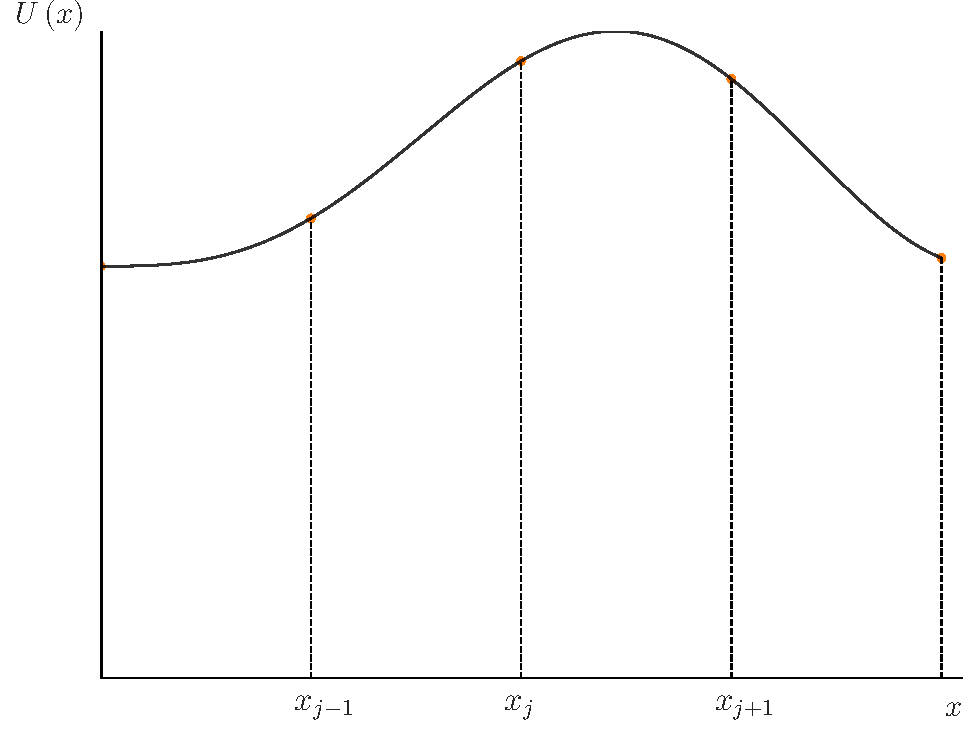
\includegraphics[width=.45\paperwidth]{discretization}
	\caption{Discretización de una función.}
	\label{fig:discretization}
\end{figure}

Para esto, el método de volúmenes finitos se reduce a la forma
conservativa de la ecuación a resolver, luego discretiza los flujos
para determinar la evolución del sistema.
Por ejemplo, considere una \emph{ley de conservación} sujeto a
condiciones iniciales y/o de fronteras.

\begin{equation}\label{eq:conservationlaw}
	\diffp{U}{t}+
	\diffp{
		f
		\left(U\right)
	}{x}=
	0
\end{equation}


\begin{enumerate}
	\item

	      Si el flujo
	      \begin{math}
		      f
		      \left(U\right)=
		      cU
	      \end{math}
	      es \emph{advectivo}, entonces~\eqref{eq:conservationlaw} es
	      la ecuación de advección lineal.

	\item


	      Si el flujo
	      \begin{math}
		      f
		      \left(U\right)=
		      -\alpha\diffp{U}{x}
	      \end{math}
	      es \emph{difusivo}, entonces~\eqref{eq:conservationlaw} es
	      la ecuación de difusión lineal.

	\item

	      Si el flujo
	      \begin{math}
		      f
		      \left(U\right)=
		      cU-
		      \alpha\diffp{U}{x}
	      \end{math},
	      entonces~\eqref{eq:conservationlaw} es la ecuación de
	      advección-difusión lineal.
\end{enumerate}

Integramos esta ecuación (para encontrar su ``forma conservativa'')
en un volumen de control, que en dimensión $1$ es solo un segmento
centrado alrededor de
\begin{math}
	x_{j}=
	j\Delta x
\end{math},
donde $\Delta x$ es el tamaño de las celdas de la malla.
Los extremos de este segmento son $x_{j-\frac{1}{2}}$ y
$x_{j+\frac{1}{2}}$; aquí el índice $\frac{1}{2}$ nos dice que estos
dos puntos están en la interfaz con celdas vecinas centradas en
$x_{j-1}$ y $x_{j+1}$.
En lugar de considerar como antes el valor tomado por $U$ en $x=x_{j}$,
introducimos el valor promedio de $U$ en el segmento
\begin{math}
	\mathcal{C}_{j}=
	\left[
		x_{j-\frac{1}{2}},
		x_{j+\frac{1}{2}}
		\right]
\end{math}:

\begin{equation*}
	U^{n}_{j}=
	\dfrac{1}{\Delta x}
	\int_{\mathcal{C}_{j}}
	U
	\left(x,t^{n}\right)
	\dl x.
\end{equation*}

\begin{figure}[ht!]
	\centering
	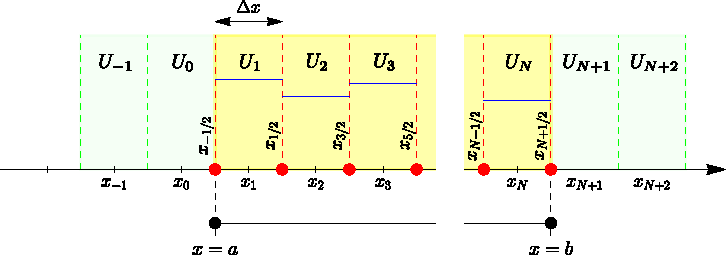
\includegraphics[width=.5\paperwidth]{computationalgrid}
	\caption{Malla computacional.
		El área de color amarillo representa el dominio computacional
		$\left[a,b\right]$, mientras que el área de color verde
		representa el dominio extendido para manejar las condiciones de
		frontera.
		El dominio computacional se puede extender mediante la inclusión
		de \emph{celdas fantasmas}.
	}
	\label{fig:piecewise}
\end{figure}

\begin{figure}[ht!]
	\centering
	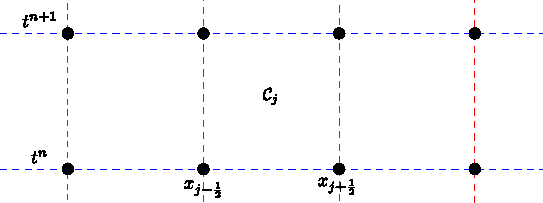
\includegraphics[width=.5\paperwidth]{computationaldomainfinitevolume}
	\caption{Dominio computacional y la malla en el plano $x-t$.}
	\label{fig:computationaldomainfinitevolume}
\end{figure}

La ventaja de esta discretización frente a las técnicas de
diferencias finitas es que el método es \emph{conservativo}, es
decir, los flujos (que expresan balances de masa, cantidad de
movimiento, etc.) se describen correctamente.

\begin{figure}[ht!]
	\centering
	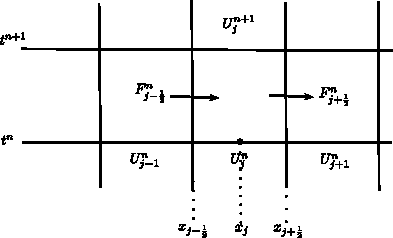
\includegraphics[width=.5\paperwidth]{finitevolumediagram}
	\label{fig:finitevolumediagram}
	\caption{Plano $x-t$ y el flujo entre las celdas.}
\end{figure}

Integramos~\eqref{eq:conservationlaw} sobre el volumen de control
\begin{math}
	\left[
		x_{j-\frac{1}{2}},
		x_{j+\frac{1}{2}}
		\right]\times
	\left[
		t^{n},
		t^{n+1}
		\right]
\end{math}.
Comencemos integrando con respecto a la variable espacial $x$.
Como la cuadrícula es fija podemos invertir las operaciones de
diferenciación:

\begin{equation*}
	\int_{C_{j}}
	\diffp{U}{t}
	\dl x=
	\diffp{}{t}
	\int_{\mathcal{C}_{j}}
	U\dl x.
\end{equation*}

También tenemos:

\begin{equation*}
	\int_{\mathcal{C}_{j}}
	\diffp{U}{x}
	f\left(U\right)
	\dl x+
	{
	\left[
		f\left(U\right)
		\right]
	\Bigr|
	}_{x_{j-\frac{1}{2}}}^{x_{j+\frac{1}{2}}}
	=0.
\end{equation*}

Por tanto, la integración de~\eqref{eq:conservationlaw} sobre
$\mathcal{C}_{j}$ es

\begin{equation*}
	\diff{}{t}
	\int_{\mathcal{C}_{j}}
	U\left(x,t\right)
	\dl x=
	f\left(U\left(x_{j-\frac{1}{2}},t\right)\right)-
	f\left(U\left(x_{j+\frac{1}{2}},t\right)\right).
\end{equation*}

Una integración con respecto al tiempo entre los tiempos $t^{n}$ y
$t^{n+1}$ proporciona la ecuación

\begin{equation*}
	\int_{\mathcal{C}_{j}}
	U
	\left(x,t^{n+1}\right)
	\dl x-
	\int_{\mathcal{C}_{j}}
	U
	\left(x,t^{n}\right)
	\dl x=
	\int_{t^{n}}^{t^{n+1}}
	\left[
		f\left(U\left(x_{j-\frac{1}{2}},t\right)\right)-
		f\left(U\left(x_{j+\frac{1}{2}},t\right)\right)
		\right]\dl t,
\end{equation*}

que también se puede escribir en la forma

\begin{equation*}
	\boxed{
		U^{n+1}_{j}=
		U^{n}_{j}-
		\frac{\Delta t}{\Delta x}
		\left(
		F^{n}_{j+\frac{1}{2}}-
		F^{n}_{j-\frac{1}{2}}
		\right),
	}
\end{equation*}

donde introdujimos el flujo promedio (a lo largo del tiempo)

\begin{equation*}
	F^{n}_{j\pm\frac{1}{2}}=
	\frac{1}{\Delta t}
	\int_{t^{n}}^{t^{n+1}}
	f\left(U\left(x_{j\pm\frac{1}{2}}\right),t\right)
	\dl t,
\end{equation*}

con tamaño de paso temporal $\Delta t=t^{n+1}-t^{n}$.
Todo el desafío de los MVF será encontrar una aproximación del flujo
promedio
\begin{math}
	F^{n}_{j+\frac{1}{2}}
\end{math}
en la interfaz entre dos celdas (vea la
Figura~\ref{fig:computationaldomainfinitevolume}).
Uno de los MVF es el esquema de \emph{Lax-Friedrichs}, que consiste
en definir una función de flujo numérico de la siguiente manera:

\begin{equation*}
	F^{n}_{j+\frac{1}{2}}=
	\frac{1}{2}
	\left[
		f\left(U^{n}_{j+1}\right)-
		f\left(U^{n}_{j}\right)-
		\frac{\Delta x}{\Delta t}
		\left(
		U^{n}_{j+1}-
		U^{n}_{j}
		\right)
		\right].
\end{equation*}

Este esquema es similar a una discretización numérica de la ecuación
de advección no lineal con un término difusivo

\begin{equation*}
	\diffp{U}{t}+
	\diffp{f\left(U\right)}{x}=
	\beta
	\diffp[2]{U}{x},
\end{equation*}

con
\begin{math}
	\beta=
	\frac{{\left(\Delta x\right)}^{2}}{2\Delta t}
\end{math}.

El término difusivo adicional comparado con la ecuación
original~\eqref{eq:conservationlaw} sirve para estabilizar la
solución numérica, sirviendo aquí la difusión para atenuar cualquier
inestabilidad que aparecería.

Posteriormente veremos esquemas que son mucho más eficientes que el
esquema Lax-Friedrichs, que introduce demasiada difusión numérica.
Estos esquemas explotan características específicas de las ecuaciones
hiperbólicas, en particular el shock y la propagación de información.

Consideremos una ecuación hiperbólica en una dimensión espacial y en
su forma conservativa.

\begin{equation}\label{eq:hyperbolic1d}
	\diffp{\bm{U}}{t}+
	\diffp{\bm{f}\left(\bm{U}\right)}{t}=
	0,
\end{equation}

donde $U\in\mathbb{R}^{m}$ y $\bm{f}$ es la función flujo.

Consideramos una cuadrícula uniforme sobre un intervalo
$\left[a,b\right]$ dividida en $N$ celdas idénticas de tamaño
\begin{math}
	\Delta x=
	\dfrac{b-a}{N}
\end{math}.

Los centros de las celdas se denotan por $x_{j-\frac{1}{2}}$

\begin{equation*}
	x_{j}=
	a+
	\left(
	j-
	\frac{1}{2}
	\right)
	\Delta x.
\end{equation*}

Definimos la celda
\begin{math}
	\mathcal{C}_{i}=
	\left[
		x_{j-\frac{1}{2}},
		x_{j+\frac{1}{2}}
		\right]
\end{math},
centrada alrededor de la celda $x_{j}$ y cuyos límites (o interfaces)
son $x_{j\pm\frac{1}{2}}$.
Note que
\begin{equation*}
	x_{-\frac{1}{2}}=
	a,
	\quad
	x_{N+\frac{1}{2}}=
	b.
\end{equation*}

El tamaño de paso es denotado por $\Delta t=t^{n+1}-t^{n}$.
El dominio computacional es $\left[a,b\right]$

\begin{equation*}
	\int_{
		x_{j-\frac{1}{2}}
	}^{
		x_{j+\frac{1}{2}}
	}
	\diffp{\bm{U}}{t}
	\dl x+
	\left[
		\bm{f}
		\left(\bm{U}\right)
		\right]
	=0.
\end{equation*}

Integrating this equation again over
\begin{math}
	\left(
	t_{n},
	t_{n+1}
	\right]
\end{math}
gives:

\begin{equation*}
	\int_{
		x_{j-\frac{1}{2}}
	}^{
		x_{j+\frac{1}{2}}
	}
	\left(
	U
	\left(x,t^{n+1}\right)-
	U
	\left(x,t^{n}\right)
	\right)
	\dl x+
	\int_{t^{n}}^{t^{n+1}}
	\left[
		\bm{f}
		\left(\bm{U}\right)
		\right]
	\dl t=
	0.
\end{equation*}

\begin{equation*}
	U^{n}_{i}=
	\frac{1}{\Delta x}
	\int_{
		x_{j-\frac{1}{2}}
	}^{
		j+\frac{1}{2}
	}
	\bm{U}
	\left(x,t^{n}\right)
	\dl x.
\end{equation*}

\begin{equation*}
	\bm{F}^{n}_{j\pm\frac{1}{2}}=
	\frac{1}{\Delta t}
	\int_{t^{n}}^{t^{n+1}}
	\bm{f}
	\left(\bm{U}\left(x_{j\pm\frac{1}{2}}\right),t\right)
	\dl t.
\end{equation*}

Posteriormente veremos esquemas que son mucho más eficientes que el
esquema Lax-Friedrichs (LxF), que introduce demasiada difusión
numérica.
Estos esquemas explotan las características específicas de las
ecuaciones hiperbólicas, en particular el shock y la propagación de
información.

\subsubsection*{Esquema de Godunov}

A finales de la década de $1950$,
Godunov\footnote{Sergei Konstantinovich Godunov~(1929-2023) fue un
	matemático miembro de la Academia de Ciencias de Rusia y profesor
	del Instituto Sobolev de Matemáticas de Novosibirsk.
	El mayor avance realizado por Godunov fue proponer un método
	compatible con la propagación de discontinuidades.} propuso un
algoritmo para resolver sistemas EDPs lineales hiperbólicas.
La idea básica explotada por Godunov es

\begin{description}
	\item[Reconstrucción]

	      Asuma que podemos aproximar la solución
	      \begin{math}
		      U
		      \left(x,t\right)
	      \end{math}
	      por una función constante a trozos
	      \begin{math}
		      \widetilde{U}^{n}_{j}
		      \left(x,t^{n}\right)=
		      U^{n}_{j}
	      \end{math}
	      en $x\in\mathcal{C_{i}}$.
	      %del dominio de cálculo y en el tiempo $t^n$, a
	      % partir de los valores promedio de las celdas
	      % (obtenidos en el paso 3 de promediar en $t^{n}$).
	      La más sencilla es considerar funciones constantes por partes
	      (esquema de Godunov de primer orden):

	      \begin{align*}
		      U^{n}_{j}
		       & =
		      \frac{1}{\Delta x}
		      \int_{x_{i-\frac{1}{2}}}^{i+\frac{1}{2}}
		      \widetilde{U}
		      \left(x,t^{n}\right)
		      \dl x, \\
		       & =
		      \frac{1}{\Delta x}
		      \int_{x_{i}-\frac{\Delta x}{2}}^{x_{i}+\frac{\Delta x}{2}}
		      \left[
			      \widetilde{U}
			      \left(x_{j},t^{n}\right)+
			      \left(x-x_{i}\right)
			      \diffp{U\left(x_{j},t^{n}\right)}{x}+
			      \frac{{\left(x-x_{j}\right)}^{2}}{2}
			      \diffp[2]{U\left(x_{j},t^{n}\right)}{x}
			      \right]
		      \dl x. \\
		       & =
		      U\left(x_{j},t^{n}\right)+
		      \frac{{\left(\Delta x\right)}^{2}}{24}
		      \diffp[2]{U\left(x_{j},t^{n}\right)}{x}
	      \end{align*}

	      % para
	      % \begin{math}
	      %   x_{j-\frac{1}{2}}\leq
	      %   x\leq
	      %   x_{j+\frac{1}{2}}
	      % \end{math}.
	      Esto nos permite considerar que en cada paso de tiempo y en cada interfaz entre dos celdas,
	      resolvemos un problema de Riemann.
	      Naturalmente, es posible considerar formas de reconstrucción más complejas,
	      por ejemplo considerando funciones lineales por partes.
	      Esto es lo que se hace con los llamados \emph{métodos de alta resolución}.

	\item[Evolución]

	      Propagación de las discontinuidades en las interfaces $x_{j-\frac{1}{2}}$ tomando como condición inicial los valores
	      \begin{math}
		      \widetilde{U}
		      \left(x,t^{n}\right)
	      \end{math}.
	      Por ejemplo, podemos utilizar el método descrito en la ecuación (3.3). Deducimos U (x, tn+1):

	\item[Promedio]

	      Promediar las funciones alteradas por el paso de las discontinuidades

	      \begin{equation*}
		      U^{n+1}_{j}=
		      \frac{1}{\Delta x}
		      \int_{x_{i-\frac{1}{2}}}^{x_{i+\frac{1}{2}}}
		      \widetilde{U}
		      \left(x,t^{n+1}\right)
		      \dl x.
	      \end{equation*}
\end{description}

\begin{figure}[ht!]
	\centering
	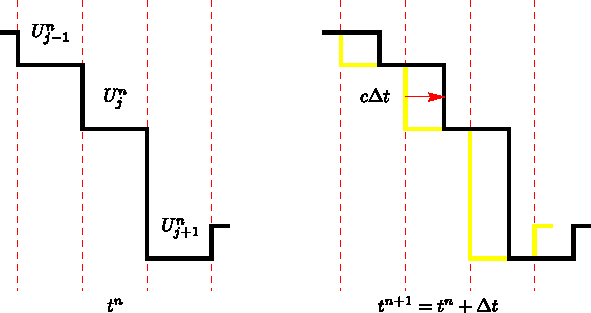
\includegraphics[width=.5\paperwidth]{piecewise}
	\caption{Advección de una función continua por partes.
	En el tiempo $t^{n}$, la función constante a trozos con valor $U^{n}_{j}$ en la celda $\mathcal{C}_{j}$.
	En el tiempo $t^{n+1}$, la función se ha desplazado en $c\Delta t$.
	El valor $U^{n+1}_{j}$ se obtiene promediando espacialmente desplazada en la celda $\mathcal{C}_{j}$.
	El problema puede interpretarse como la propagación de discontinuidades que se originan en el extremo
	$x_{j-\frac{1}{2}}$.
	Estas discontinuidades forman la onda $W_{i-\frac{1}{2}}=U_{j}-U_{j-1}$.}
	\label{fig:piecewise}
\end{figure}

% Ahora veremos los principales tipos de ecuaciones diferenciales
% parciales que se encuentran en hidráulica:

% \begin{equation*}
% 	a_{j}=
% 	\dfrac{U^{n}_{j+1}-U^{n}_{j-1}}{2\Delta x}
% \end{equation*}

% \begin{equation*}
% 	a_{i}=
% 	\dfrac{U^{n}_{j}-U^{n}_{j-1}}{\Delta x}
% \end{equation*}

% \begin{equation*}
% 	a_{i}=
% 	\dfrac{U^{n}_{j+1}-U^{n}_{j}}{\Delta x}.
% \end{equation*}

% \begin{equation*}
% 	a_{i}=
% 	\operatorname{minmod}
% 	\left(
% 	\dfrac{U^{n}_{j}-U^{n}_{j-1}}{\Delta x},
% 	\dfrac{U^{n}_{j+1}-U^{n}_{j}}{\Delta x}
% 	\right)
% \end{equation*}
% Por fenómenos
% \begin{itemize}
% 	\item

% 	      transporte por convección (o advección);

% 	\item

% 	      transporte por difusión;

% 	\item

% 	      fenómenos ondulatorios;

% 	\item

% 	      fenómenos de equilibrio.
% \end{itemize}


% \section*{Apéndice}
% \addcontentsline{toc}{section}{Apéndice}
% %
% When placed at se \textit{do not} use the \verb|appendix| command when

% \begin{equation}
% 	a \times b = c
% \end{equation}
% % Problems or Exercises should be sorted chapterwise
% \section*{Problemas}
% \addcontentsline{toc}{section}{Problemas}
% %
% % Use the following environment.
% % Don't forget to label each problem;
% % the label is needed for the solutions' environment
% \begin{prob}
%     \label{prob1}
%     A given problem or Excercise is described here. The
%     problem is described here. The problem is described here.
% \end{prob}

% \begin{prob}
%     \label{prob2}
%     \textbf{Problem Heading}\\
%     (a) The first part of the problem is described here.
% \end{prob}

\section{Esquema conservativo con limitador de pendiente}

\section*{Funciones limitadores de pendiente}

La idea básica detrás del concepto de limitadores fue concebido
por~\cite{vanLeer2003} para controlar el proceso de la generación de
los sobreimpulsos y subimpulsos en los métodos de diferencias finitas
de orden mayor o igual que dos sujeto a condiciones iniciales
discontinuas.

Para problemas que dependen del tiempo, en particular para
problemas de Riemann, se agrega restricciones a los esquemas numéricos
para permitir el seguimiento de las discontinuidades en tiempos largos.
Para ilustrar la idea detrás de los limitadores, considere la
ecuación de transporte $\difcp{u}{t}+a\difcp{u}{x}=0$, siendo $a>0$.
\begin{equation*}
	\diff{u_{i}}{t}=
	-\frac{a}{2\Delta x}
	\left(u_{i+1}-u_{i-1}\right)=
	-\frac{a}{2\Delta x}
	\left[
		-\left(u_{i-1}-u_i\right)+
		\left(u_{i+1}-u_i\right)
		\right].
\end{equation*}
En el último término podemos ver que uno de los coeficientes es
negativo, lo que indica que este esquema no es monótono.
Dado que el concepto de limitadores se basa en el monitoreo de la
relación de gradientes sucesivos, escribimos el esquema anterior
bajo la forma
\begin{equation*}
	\diff{u_{i}}{t}=
	-\frac{a}{2\Delta x}
	\left[
	1-\frac{u_{i+1}-u_i}{u_i-u_{i-1}}
	\right]
	\left(u_i-u_{i-1}\right).
\end{equation*}
Observamos que este esquema podría volverse monótono si el término
entre corchetes permaneciera positivo, es decir, si la relación entre
gradientes sucesivos permanece menor que 1.
\begin{equation*}
	r_{i}=
	\frac{u_{i+1}-u_i}{u_i-u_{i-1}}\leq
	1.
\end{equation*}

La metodología se define como sigue
\begin{enumerate}
	\item

	      Seleccione una discretización espacial monótona de primer
	      orden, por ejemplo Upwind, y escriba el esquema de orden
	      superior como el esquema monótono más términos adicionales.

	\item

	      Multiplique los términos adicionales por una función
	      limitadora, expresada como una función de la razón de
	      gradientes sucesivos.

	\item

	      Exprese las condiciones de monotonía para derivar las
	      condiciones de los limitadores.
\end{enumerate}

Para ilustrar la idea detrás de los limitadores, considere una
diferencia hacia atrás de segundo orden para la ecuación de
transporte $\difcp{u}{t}+a\difcp{u}{x}=0$, siendo $a>0$.
\begin{align*}
	\diff{u_{i}}{t} & =
	-\frac{a}{2\Delta x}
	\left(3u_{i}-4u_{i-1}+u_{i-2}-\right)=
	-\frac{a}{2\Delta x}
	\left[
		3\left(u_{i}-u_{i-1}\right)-
		\left(u_{i-1}-u_{i-2}\right)
	\right].            \\
	                & =
	-\frac{a}{2\Delta x}
	\left[
		-4\left(u_{i-1}-u_{i}\right)+
		\left(u_{i-2}-u_{i}\right)
		\right].
\end{align*}
En la último igualdad podemos ver que uno de los coeficientes es
negativo, lo que indica que este esquema no es monótono.
Apliquemos la metodología propuesta, paso a paso.
\begin{description}
	\item[Primer paso]

	      Reescriba el esquema como una corrección
	      del esquema FOU, escribiendo los términos de corrección como
	      una diferencia de gradientes.
	      \begin{equation*}
		      \diff{u_{i}}{t}=
		      \underbrace{
			      -\frac{a}{\Delta x}
			      \left(u_i-u_{i-1}\right)}_{\text{Esquema FOU}}-
		      \frac{a}{\Delta x}
		      \left[
			      +\frac{1}{2}
			      \left(u_i-u_{i-1}\right)-
			      \frac{1}{2}
			      \left(u_{i-1}-u_{i-2}
			      \right)
			      \right].
	      \end{equation*}


	\item[Segundo paso]

	      Multiplica los dos términos no monótonos por las funciones
	      $\Psi\left(r_{i}\right)$ y $\Psi\left(r_{i-1}\right)$, donde
	      \begin{equation*}
		      r_{i-1}=
		      \frac{u_{i}-u_{i-1}}{u_{i-1}-u_{i-2}}\quad
		      r_i=\frac{u_{i+1}-u_i}{u_i-u_{i-1}}.
	      \end{equation*}
	      que conduce a
	      \begin{align*}
		      \diff{u_{i}}{t} & =
		      -\frac{a}{\Delta x}
		      \left[
			      \left(u_{i}-u_{i-1}\right)+
			      \frac{1}{2}
			      \Psi\left(r_{i}\right)
			      \left(u_{i}-u_{i-1}\right)-
			      \frac{1}{2}
			      \Psi\left(r_{i-1}\right)
			      \left(u_{i-1}-u_{i-2}\right)
		      \right]             \\
		                      & =
		      -\frac{a}{\Delta x}
		      \left[
			      1+
			      \frac{1}{2}
			      \Psi\left(r_{i}\right)-
			      \frac{1}{2}
			      \frac{\Psi\left(r_{i-1}\right)}{r_{i-1}}
			      \right]
		      \left(
		      u_{i}-u_{i-1}
		      \right)
	      \end{align*}

	\item[Tercer paso]
	      Derive las condiciones sobre los limitadores.

	      Este esquema será monótono si el término entre paréntesis es
	      positivo, es decir, los limitadores deben satisfacer la
	      condición.
	      \begin{equation*}
		      \frac{\Psi\left(r_{i-1}\right)}{r_{i-1}}-\Psi\left(r_{i}\right)\leq
		      2.
	      \end{equation*}
\end{description}

\subsection{Aplicación de las funciones limitadoras}

Ahora presentamos una aplicación del uso de la funciones limitadores para el esquema
Second Order Upwind (SOU) y Beam-Warming.
Consideramos el Beam-Warming definido por
\begin{equation*}
	u_{i}^{n+1}=
	u_{i}^{n}+
	\sigma(2-\sigma)
	\left(u_{i-1}^n-u_i^n\right)+
	\frac{\sigma}{2}(\sigma-1)
	\left(u_{i-2}^{n}-u_{i}^{n}\right)
\end{equation*}

\begin{description}
	\item[Paso 1]
	      Reescriba el esquema como una corrección al esquema FOU, con los
	      términos adicionales bajo la forma de diferencias entre puntos adyacentes
	      \begin{equation*}
		      u_{i}^{n+1}=
		      \underbrace{
			      u_{i}^{n}-
			      \sigma\left(u_i^n-u_{i-1}^n\right)}_{\text{Esquema Monótono}}-
		      \underbrace{
			      \frac{\sigma}{2}
			      \left(1-\sigma\right)
			      \left(u_{i}^{n}-u_{i-1}^{n}\right)+
			      \frac{\sigma}{2}
			      \left(1-\sigma\right)
			      \left(u_{i-1}^{n}-u_{i-2}^{n}\right)}_{\text {Términos no monótonos}}
	      \end{equation*}

	\item[Paso 2]

	      Multiplique los dos términos no monótonos por las funciones
	      $\Psi\left(r_{i}\right)$ y $\Psi\left(r_{i-1}\right)$,
	      lo que resulta en
	      \begin{align*}
		      u_{i}^{n+1} & =
		      u_{i}^{n}-
		      \sigma\left(u_i^n-u_{i-1}^n\right)-
		      \frac{\sigma}{2}
		      \left(1-\sigma\right)
		      \Psi\left(r_{i}\right)
		      \left(u_{i}^{n}-u_{i-1}^{n}\right)+
		      \frac{\sigma}{2}
		      \left(1-\sigma\right)
		      \Psi\left(r_{i-1}\right)
		      \left(u_{i-1}^{n}-u_{i-2}^{n}\right).
	      \end{align*}

	\item[Paso 3]

	      Este esquema limitado será monótono si el término entre
	      corchetes es positivo, lo que lleva a la condición
	      \begin{equation*}
		      \frac{\Psi\left(r_{i-1}\right)}{r_{i-1}}-
		      \Psi\left(r_{i}\right)\leq
		      \frac{2}{1-\sigma}.
	      \end{equation*}
	      Esta relación es satisfecha con la condición
	      \begin{equation*}
		      0\leq\Psi\left(r\right)\leq
		      \min\left\{\frac{2r}{\sigma},\frac{2}{1-\sigma}\right\}.
	      \end{equation*}
\end{description}

Como segunda aplicación de la función limitadora, consideremos el
esquema de Lax-Wendroff

\begin{description}
	\item[Paso 1]

	      Reescriba el esquema Lax-Wendroff como una corrección al esquema FOU.
	      \begin{equation*}
		      u_i^{n+1}=
		      \underbrace{
		      u_i^{n}-
		      \sigma\left(u_i^n-u_{i-1}^n\right)}_{\text{Esquema monótono}}-
		      \underbrace{
			      \frac{\sigma}{2}
			      \left(1-\sigma\right)
			      \left(u_{i+1}^{n}-u_{i}^{n}\right)+
			      \frac{\sigma}{2}\left(1-\sigma\right)
			      \left(u_{i}^{n}-u_{i-1}^{n}\right)}_{\text {Términos no monótonos}}
	      \end{equation*}

	\item[Paso 2]

	      Multiplique los dos términos no monótonos por las funciones
	      $\Psi\left(R_{i}\right)$ y $\Psi\left(R_{i-1}\right)$, lo que
	      da como resultado
	      \begin{align*}
		      u_{i}^{n+1} & =
		      u_{i}^{n}-
		      \sigma\left(u_i^n-u_{i-1}^n\right)-
		      \frac{\sigma}{2}(1-\sigma)
		      \Psi\left(R_i\right)\left(u_{i+1}^n-u_i^n\right)+
		      \frac{\sigma}{2}(1-\sigma)
		      \Psi\left(R_{i-1}\right)
		      \left(u_i^n-u_{i-1}^n\right). \\
		      u_{i}^{n+1} & =
		      u_{i}^{n}-
		      \sigma\left(u_i^n-u_{i-1}^n\right)
		      \left\{
		      1+
		      \frac{1}{2}
		      (1-\sigma)
		      \left[
			      \frac{\Psi\left(R_i\right)}{R_i}-\Psi\left(R_{i-1}\right)
			      \right]
		      \right\}
		      \left(u_i^n-u_{i-1}^n\right).
	      \end{align*}

	\item[Paso 3]
	      Este esquema limitado será monótono si el término entre
	      corchetes es positivo, lo que da lugar a la condición
	      \begin{equation*}
		      \Psi\left(R_{i-1}\right)-\frac{\Psi\left(R_{i}\right)}{R_{i}}\leq
		      \frac{2}{1-\sigma}.
	      \end{equation*}
\end{description}

Todas las funciones limitadoras de pendiente presentadas a
continuación satisfacen
\begin{equation}
	\forall\theta\in
	\left(0,\theta_{\max}\right):
	\frac{\phi\left(\theta\right)}{\theta}=
	\phi
	\left(\frac{1}{\theta}\right).\tag{Simetría}
\end{equation}

Algunas de ellas son
\begin{description}
	\item[van Leer]

	      \begin{equation*}
		      \phi_{\text{vl}}
		      \left(\theta\right)=
		      \frac{\theta+\left|\theta\right|}{1+\left|\theta\right|}.
	      \end{equation*}

	\item[van Albada $1$]

	      \begin{equation*}
		      \phi_{\text{va1}}
		      \left(\theta\right)=
		      \frac{\theta^{2}+\theta}{\theta^{2}+1}.
	      \end{equation*}

	\item[van Albada $2$]

	      \begin{equation*}
		      \phi_{\text{va2}}
		      \left(\theta\right)=
		      \frac{2\theta}{\theta^{2}+1}.
	      \end{equation*}

	\item[Sweby]

	      \begin{equation*}
		      \phi_{\text{sw}}
		      \left(\theta\right)=
		      \max
		      \left\{
		      0,
		      \min
		      \left\{1,2\theta\right\},
		      \min
		      \left\{2,\theta\right\}
		      \right\}
	      \end{equation*}

	\item[Superbee]

	      \begin{equation*}
		      \phi_{\text{\text{sb}}}
		      \left(\theta\right)=
		      \max
		      \left(
		      0,
		      \min\left(1,2\theta\right),
		      \min\left(2,\theta\right)
		      \right)
	      \end{equation*}

	\item[Mononotized central]

	      \begin{equation*}
		      \phi_{\text{\text{mc}}}
		      \left(\theta\right)=
		      \max
		      \left\{
		      0,
		      \min
		      \left\{
		      \frac{1+\theta}{2},2\theta,2
		      \right\}
		      \right\}
	      \end{equation*}

	\item[Minmod]

	      \begin{equation*}
		      \phi_{\text{\text{mm}}}
		      \left(\theta\right)=
		      \operatorname{minmod}
		      \left(1,\theta\right),
		      % \max
		      % \left(
		      % 0,
		      % \min
		      % \left(
		      %   1,\theta
		      %   \right)
		      % \right)
	      \end{equation*}

	      donde

	      \begin{equation*}
		      \operatorname{minmod}
		      \left(a,b\right)=
		      \begin{cases}
			      \left|a\right|,
			                      & \text{si }
			      \left|a\right|<\left|b\right|
			      \text{ y }ab>0.                   \\
			      \left|b\right|, & \text{si }
			      \left|b\right|<\left|a\right|
			      \text{ y }ab>0.                   \\
			      0,              & \text{si }ab<0.
		      \end{cases}
	      \end{equation*}

	\item[Koren]

	      \begin{equation*}
		      \phi_{\text{\text{kn}}}
		      \left(\theta\right)=
		      \max
		      \left\{
		      0,
		      \min
		      \left\{
		      2\theta,
		      \min
		      \left\{
		      2,
		      \frac{1+2\theta}{3}
		      \right\}
		      \right\}
		      \right\}
	      \end{equation*}
\end{description}

\begin{figure}[ht!]
	\centering
	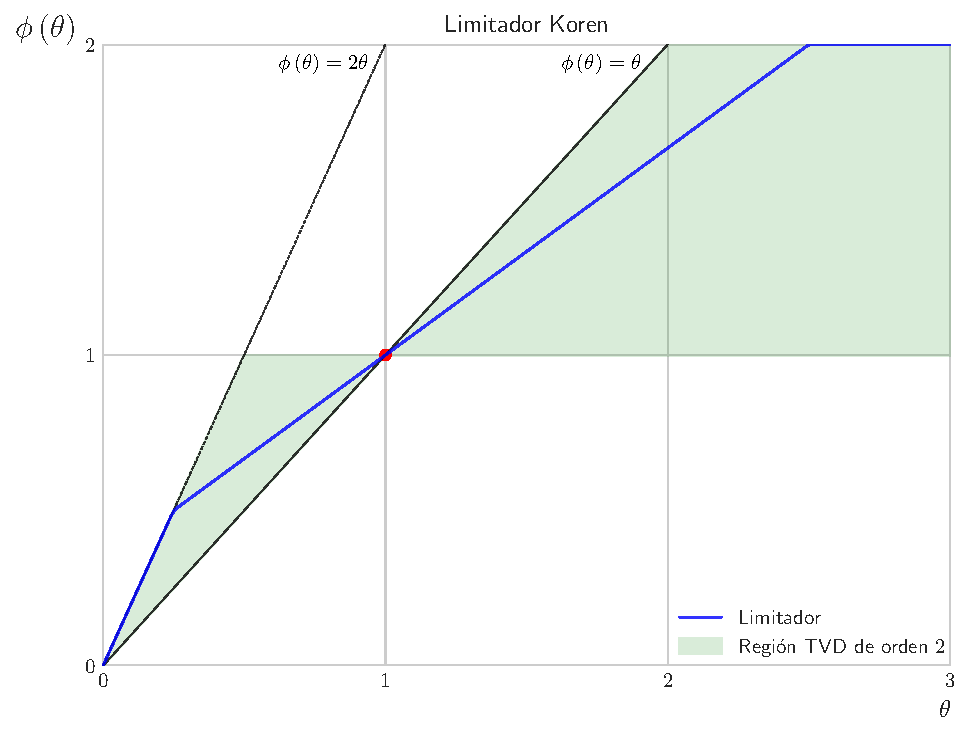
\includegraphics[width=.28\paperwidth]{limiters/limiterkoren}
	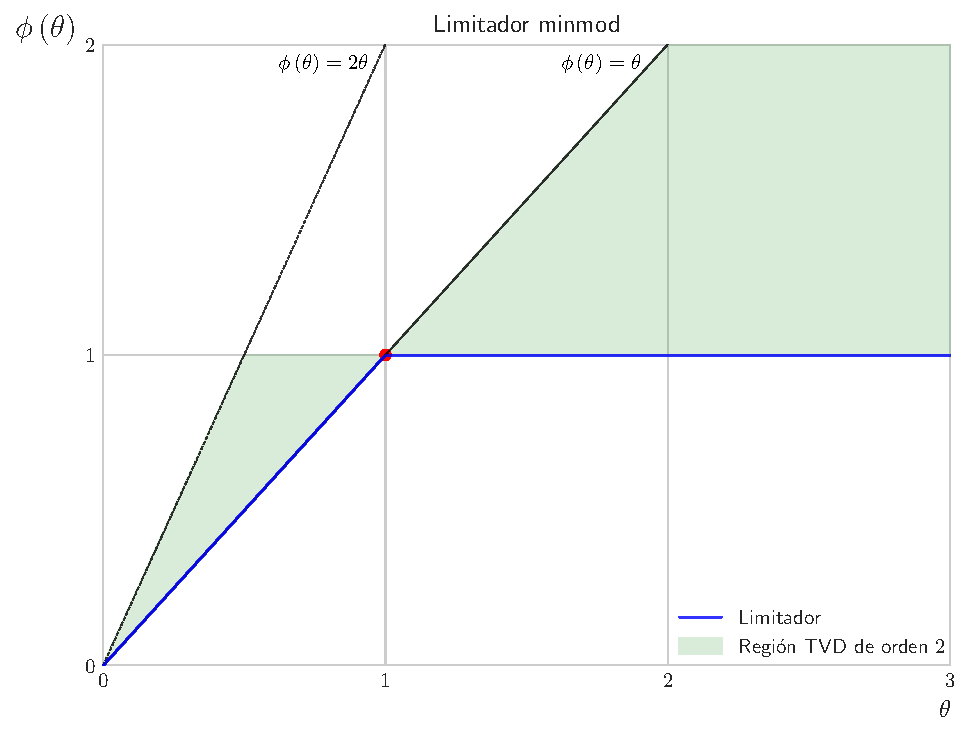
\includegraphics[width=.28\paperwidth]{limiters/limiterminmod}
	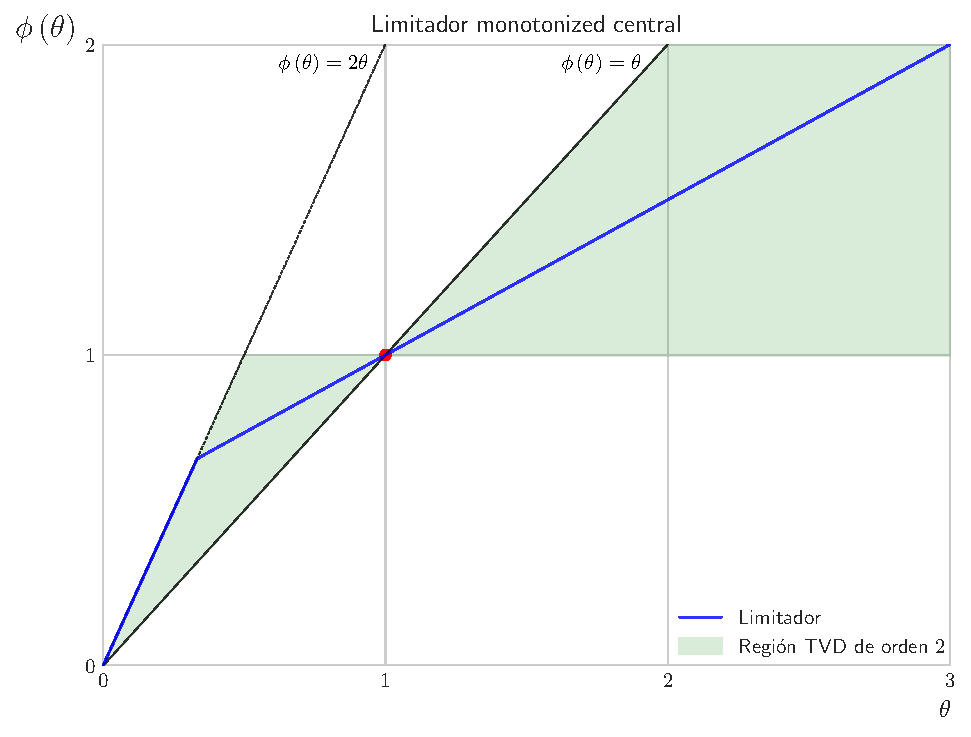
\includegraphics[width=.28\paperwidth]{limiters/limitermonotonizedcentral}
	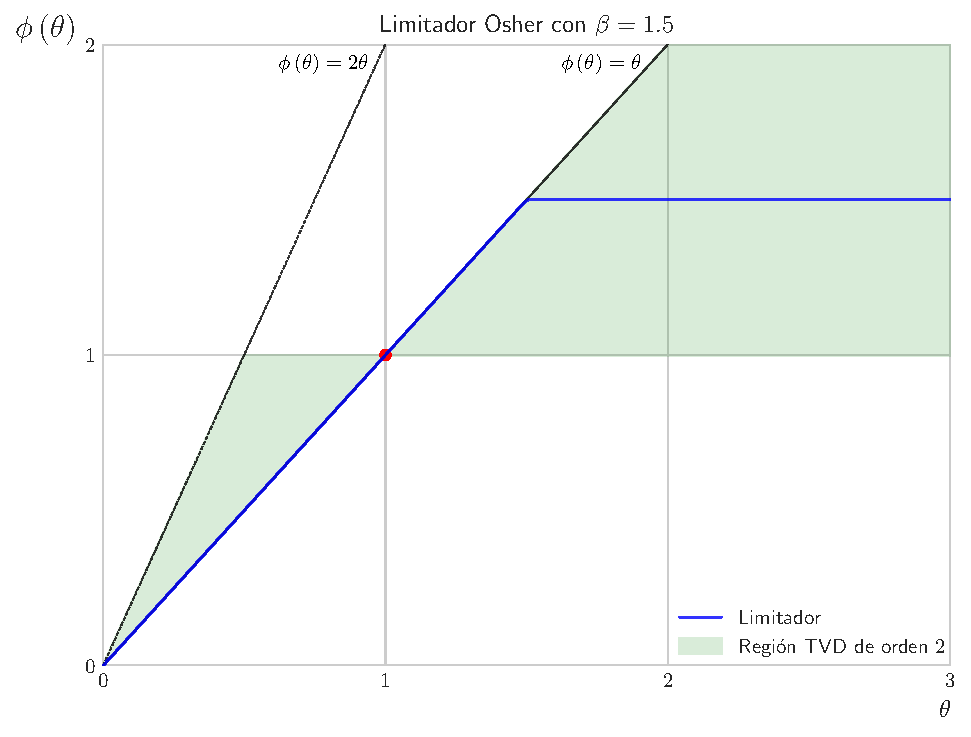
\includegraphics[width=.28\paperwidth]{limiters/limiterosher}
	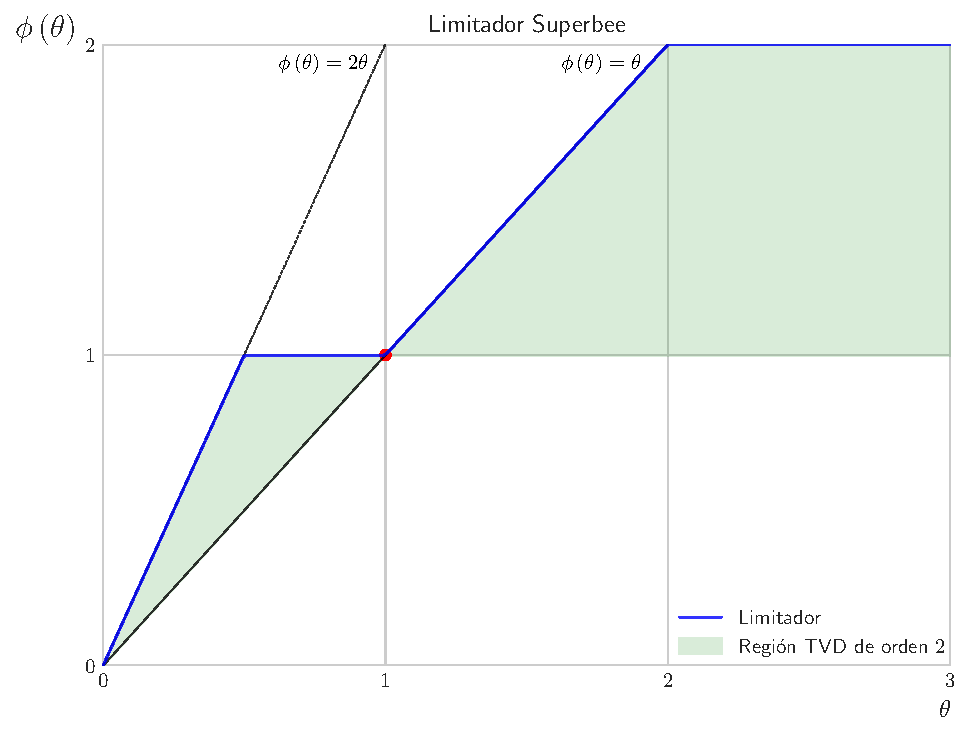
\includegraphics[width=.28\paperwidth]{limiters/limitersuperbee}
	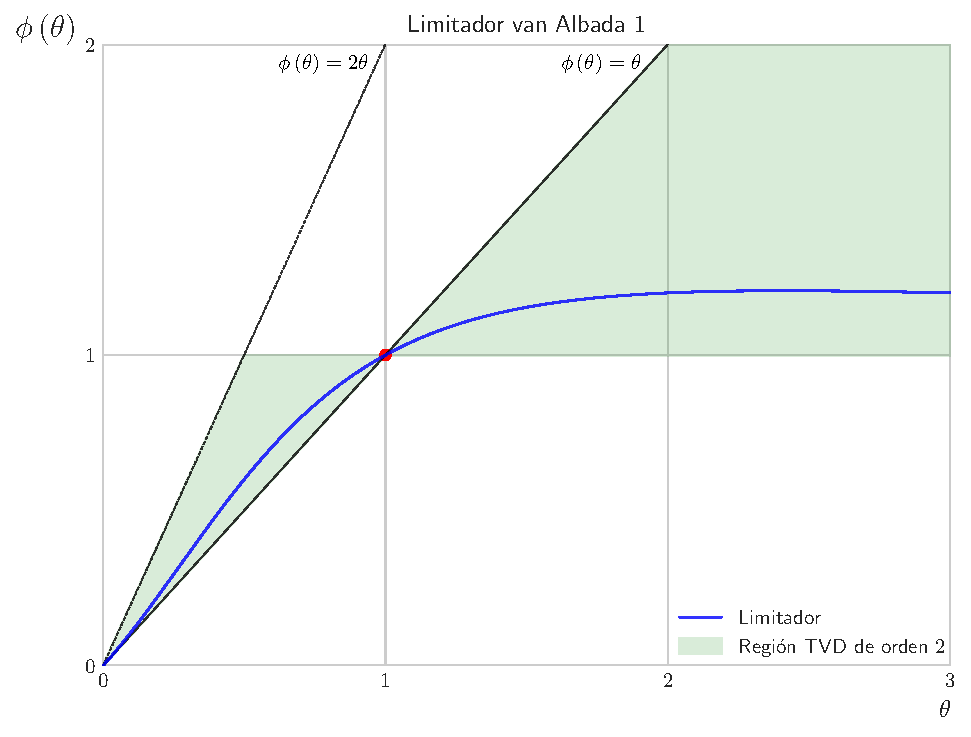
\includegraphics[width=.28\paperwidth]{limiters/limitervanalbada1}
	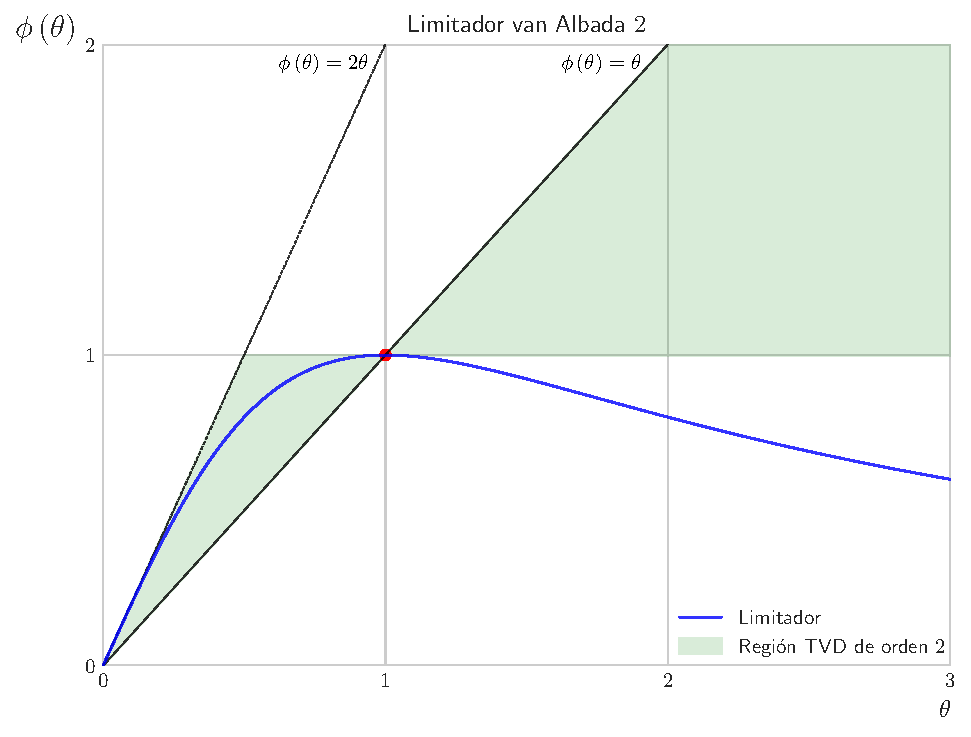
\includegraphics[width=.28\paperwidth]{limiters/limitervanalbada2}
	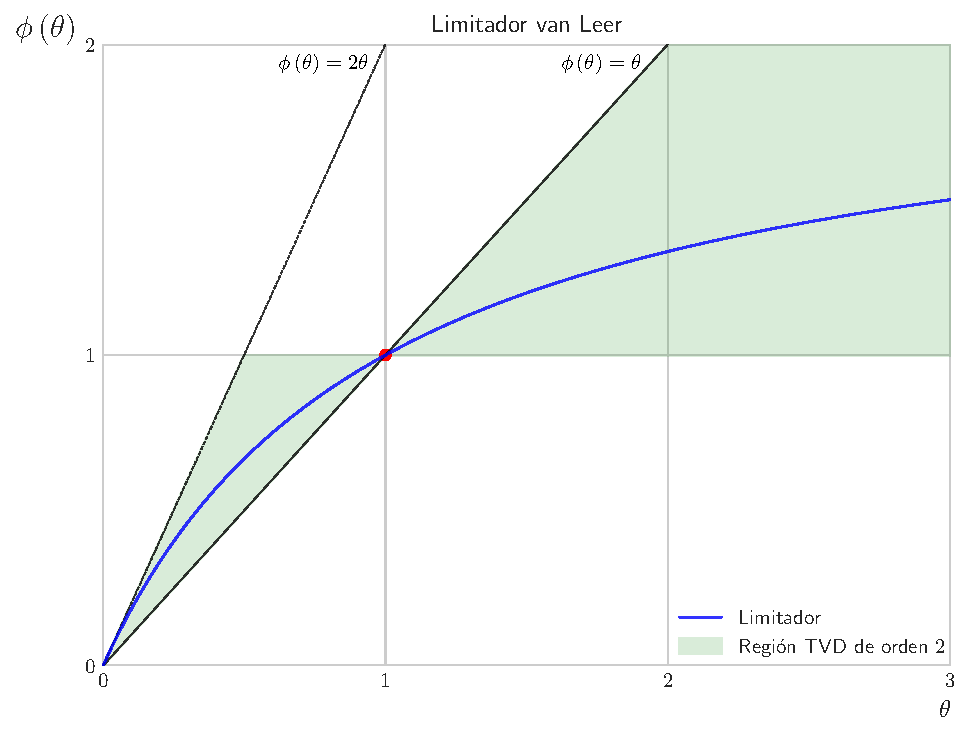
\includegraphics[width=.28\paperwidth]{limiters/limitervanleer}
	\caption{Diagrama TVD de Sweby.}
	\label{fig:slopelimiters}
\end{figure}

\section{Formulación de volúmenes finitos de esquemas y limitadores}

La formulación de volúmenes finitos de un esquema conservativo general es definido en dos componentes.
\begin{enumerate}
	\item El flujo numérico identifica completamente el esquema, ya sea en su forma explícita o
	      cuando el espacio y tiempo son discretizados por separado.
	\item
	      La definición de los valores de las caras de las celdas en función
	      de las cantidades promediadas por celda, que son las únicas
	      variables disponibles.
\end{enumerate}

Considere la ley de conservación unidimensional
\begin{math}
	\diffp{u}{t}+\diffp{f}{x}=0
\end{math}
y defina el flujo numérico en la cara de la celda $(i+\frac{1}{2})$,
como una función de los valores de la función circundante
\begin{equation*}
	f_{i+\frac{1}{2}}^{\ast}=
	f_{i+\frac{1}{2}}^{\ast}
	\left(
	u_{i},u_{i+1},u_{i-1},\dotsc
	\right)
\end{equation*}
con la condición de consistencia, que para valores iguales de $u$, el
flujo numérico debería reducirse al flujo físico $f\left(u\right)$.
Es decir,
\begin{equation*}
	f_{i+\frac{1}{2}}^{\ast}
	\left(u,u,u,\dotsc\right)=
	f\left(u\right).
\end{equation*}
El esquema de volumen finito explícito se reduce a
\begin{equation*}
	u_{i}^{n+1}=
	u_{i}^{n}-
	\frac{\Delta t}{\Delta x_{i}}
	{\left(f_{i+\frac{1}{2}}^{\ast}-f_{i-\frac{1}{2}}^{\ast}\right)}^{n}
\end{equation*}
Si mantenemos separada la integración temporal, entonces se reduce al
sistema de EDO en el tiempo
\begin{equation*}
	\diff{u_{i}}{t}=
	-\frac{1}{\Delta x_{i}}
	\left(
		f_{i+\frac{1}{2}}^{\ast}-
	f_{i-\frac{1}{2}}^{\ast}
	\right).
\end{equation*}

% Finalmente, consideremos el flujo numérico
% $f_{i+\frac{1}{2}}^{\ast}=au_{i+\frac{1}{2}}$ para esquemas explícitos

% \begin{description}
% 	\item[First Order Upwind]

% 	$u_i^{n+1}=u_i^n-\sigma\left(u_i^n-u_{i-1}^n\right)$

% \end{description}

% $u_{i+1 / 2}=u_i$


% Warming-Beam (SOU)

% $u_i^{n+1}=  u_i^n-\sigma\left(u_i^n-u_{i-1}^n\right)-\frac{\sigma}{2}(1-\sigma)\left(u_i^n-u_{i-1}^n\right)+\frac{\sigma}{2}(1-\sigma)\left(u_{i-1}^n-u_{i-2}^n\right)$

% $u_{i+1 / 2}=u_i+\frac{1}{2}(1-\sigma)\left(u_i-u_{i-1}\right)$

% Lax-Wendroff (LW)

% $u_i^{n+1}=u_i^n-\sigma\left(u_i^n-u_{i-1}^n\right)-\frac{\sigma}{2}(1-\sigma)\left(u_{i+1}^n-u_i^n\right)+\frac{\sigma}{2}(1-\sigma)\left(u_i^n-u_{i-1}^n\right)$

% $u_{i+1 / 2}=u_i+\frac{1}{2}(1-\sigma)\left(u_{i+1}-u_i\right)$

% Familia de esquemas de primer orden

% $u_i^{n+1}= u_i^n-\sigma\left(u_i^n-u_{i-1}^n\right) -\left(\frac{\sigma}{2}-\gamma\right)\left[\left(u_{i+1}^n-u_i^n\right)-\left(u_i^n-u_{i-1}^n\right)\right]$

% $u_{i+1 / 2}=u_i+\frac{1}{2}\left(1-\frac{2 \gamma}{\sigma}\right)\left(u_{i+1}-u_i\right)$

% Familia de esquemas de segundo orden

% $u_i^{n+1}= u_i^n-\sigma\left(u_i^n-u_{i-1}^n\right)-\frac{\sigma}{2}(1-\sigma)\left(u_{i+1}^n-u_i^n\right)+\frac{\sigma}{2}(1-\sigma)\left(u_i^n-u_{i-1}^n\right)+\gamma\left[\left(u_{i+1}-2 u_i+u_{i-1}\right)-\left(u_{i-2}^n-2 u_{i-1}^n+u_i^n\right)\right]$


% $u_{i+1 / 2}=u_i+\frac{1}{2}(1-\sigma)\left(u_{i+1}-u_i\right)-\frac{\gamma}{\sigma}\left[\left(u_{i+1}-u_i\right)-\left(u_i-u_{i+1}\right)\right]$

% $$
% 	\Psi(r)=\max \left[0, \min \left(\frac{2 r}{\sigma}, 1\right), \min \left(r, \frac{2}{1-\sigma}\right)\right]
% $$

% % This limiter is also considered by Leonard (1991), as part of the ultimate strategy for limiters.

% % The generalization of the ALFA family (8.3.70) to CFL dependent conditions has been initially considered by Roe and Baines (1981), and applied by Jeng and Paine (1995), Arora and Roe (1997), under the form

% $$
% 	\Psi(r)=\max \left[0, \min \left(\frac{2 r}{\sigma}, \alpha(r-1)+1, \frac{2}{1-\sigma}\right)\right]
% $$

% % where the parameter $\alpha$ can be made CFL dependent.
% % The value $\alpha=(2-\sigma) / 3$ is advocated by Arora and Roe (1997) as it corresponds to the third order scheme (8.2.49) (see Problem P.8.17). These authors also recommend to restrict the limiter region to the stationary limits $\Psi=2$ and $\Psi=2 r$ for nonlinear waves. This leads to the alternative

% $$
% 	\Psi(r)=\max [0, \min (2 r, \alpha(r-1)+1,2)] \quad \text { with } \alpha=\alpha(\sigma)
% $$

\chapter{Resultados}

Se ha considerado la resolución numérica por el método de las
funciones limitadores para la ecuación de transporte con una
condición discontinua.
En cada caso se cuenta con la solución exacta.

\begin{figure}[ht!]
	\centering
	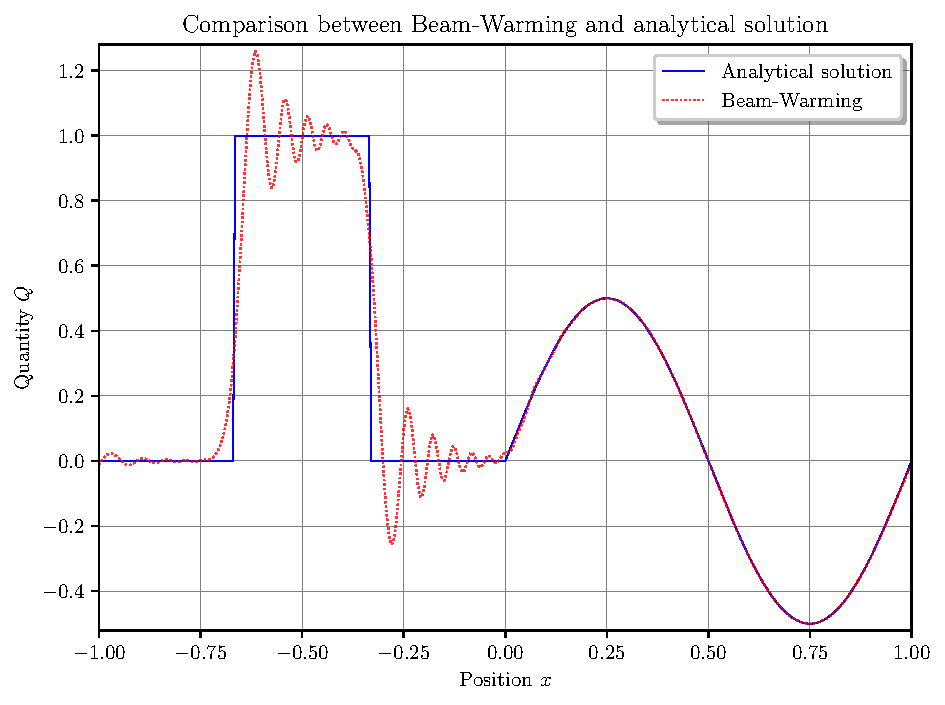
\includegraphics[width=.28\paperwidth]{graphics/Beam-Warming}
	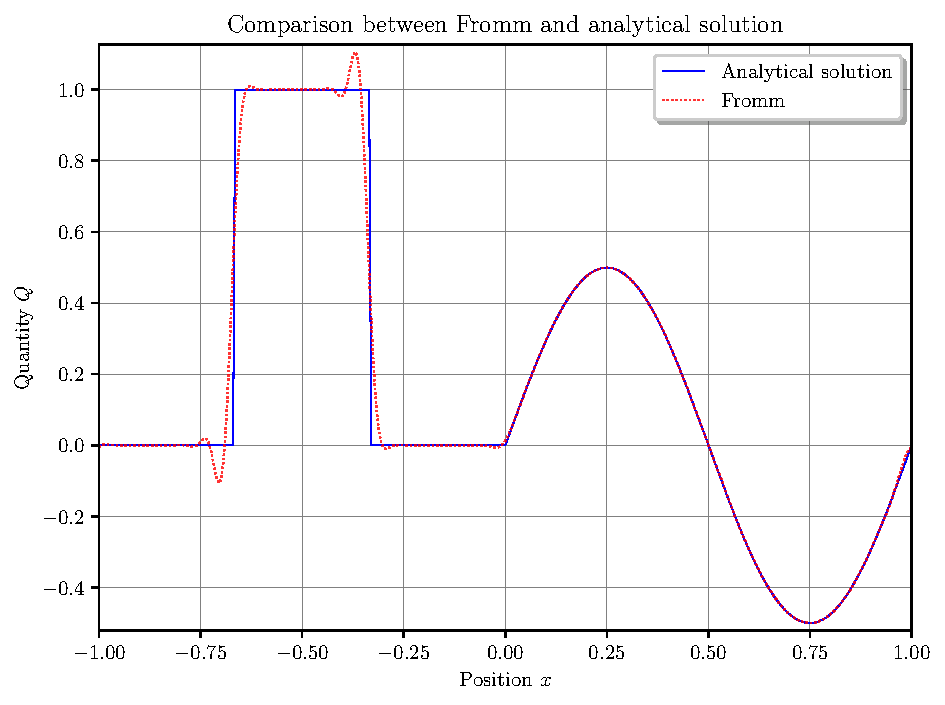
\includegraphics[width=.28\paperwidth]{graphics/Fromm}
	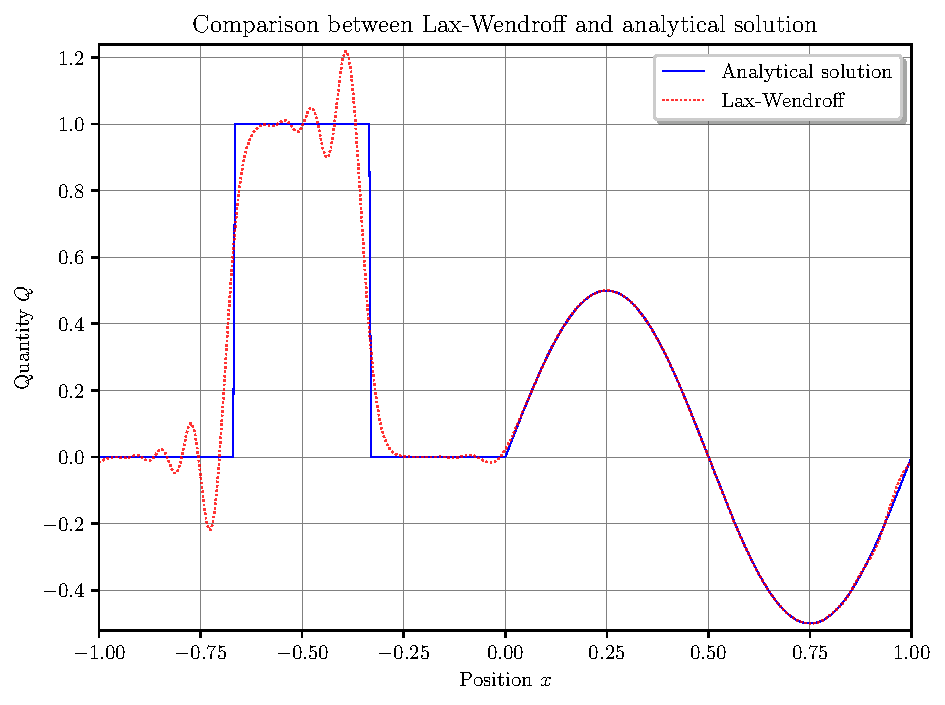
\includegraphics[width=.28\paperwidth]{graphics/Lax-Wendroff}
	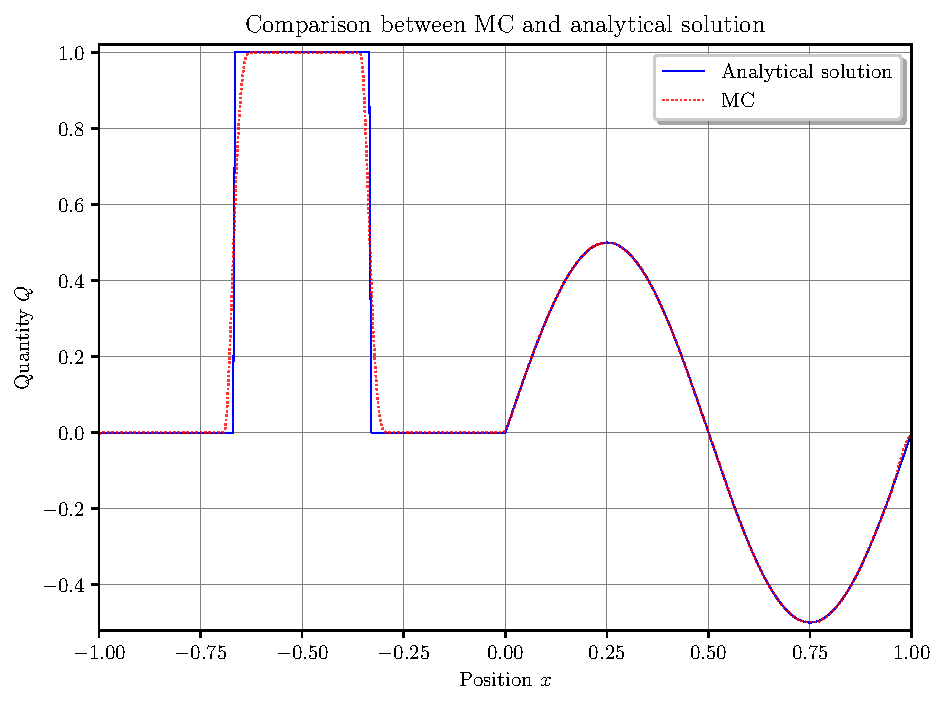
\includegraphics[width=.28\paperwidth]{graphics/MC}
	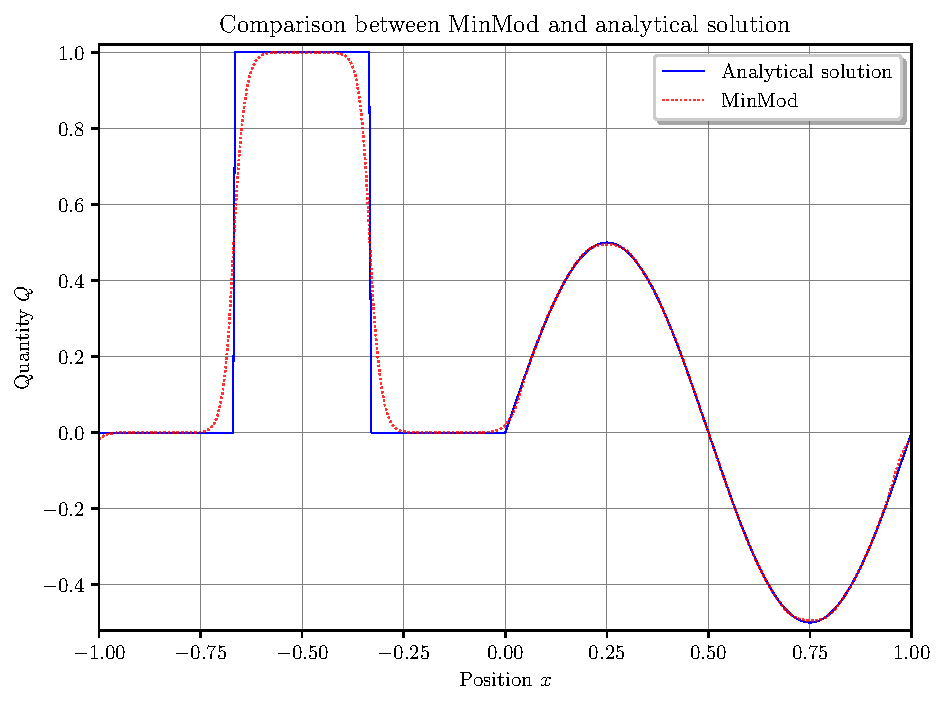
\includegraphics[width=.28\paperwidth]{graphics/MinMod}
	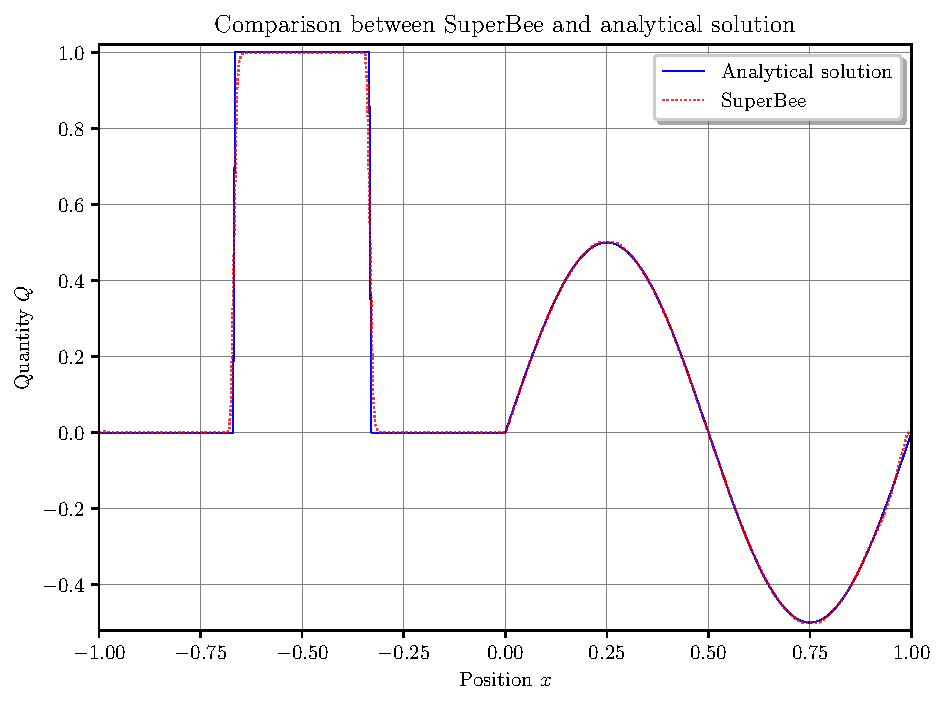
\includegraphics[width=.28\paperwidth]{graphics/SuperBee}
	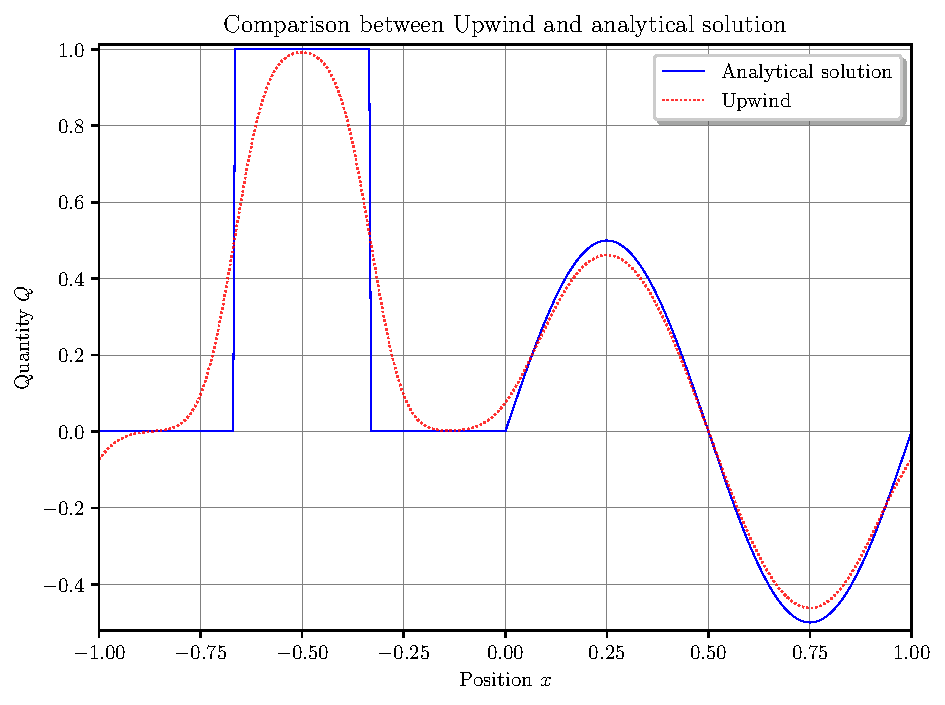
\includegraphics[width=.28\paperwidth]{graphics/Upwind}
	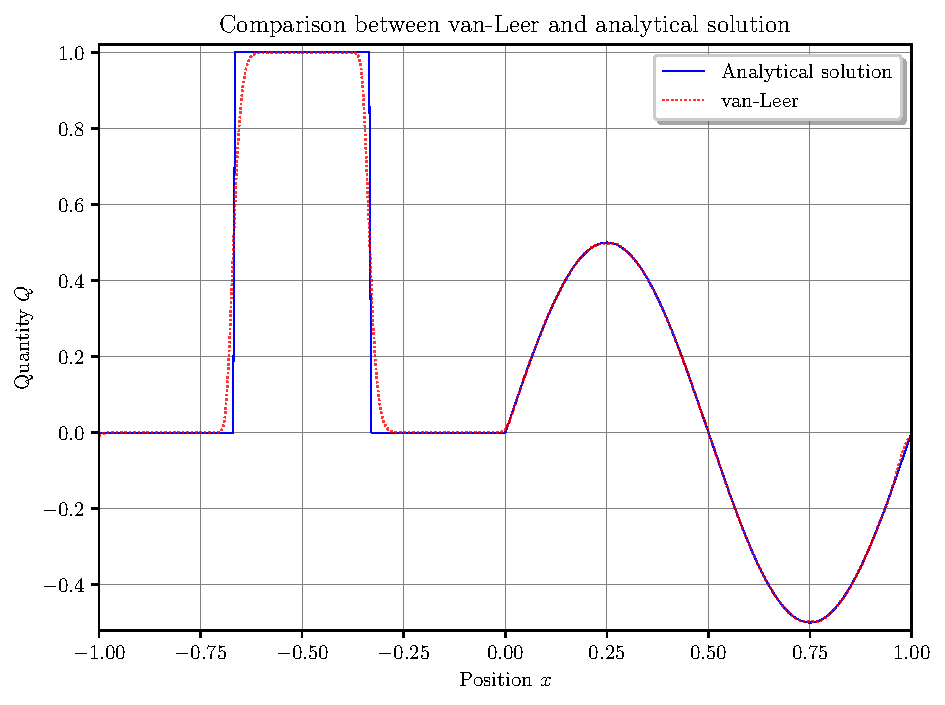
\includegraphics[width=.28\paperwidth]{graphics/van-Leer}
	\caption{De arriba hacia abajo y de izquierda a derecha.
		Se considera un perfil de onda cuadrada y sinusoidal.
		Se compara con distintas funciones limitadoras.}
\end{figure}

\cleardoublepage
\nocite{*}
\printbibliography[title={Referencias},heading=bibintoc]
